\documentclass[a4paper, 12pt]{article}
\usepackage[utf8x]{inputenc}
\usepackage[english, russian]{babel}
\usepackage[left=25mm, top=25mm, right=25mm, bottom=25mm]{geometry}
\usepackage{cmap}
\usepackage{indentfirst}
\usepackage{tikz}
\usepackage{float}
\usepackage{amsmath, amsfonts, amssymb}
\usepackage{graphicx}
\usepackage{hyperref}
\usepackage{listings}
\usepackage{caption}
\usepackage{subcaption}
\usepackage{xcolor}
\usepackage{etoolbox}
\usepackage{titlesec}
\usepackage{array}
\pagestyle{plain}
\patchcmd{\tableofcontents}{\contentsname}{\centering\contentsname}{}{}
\titleformat{\section}[block]{\normalfont\large\bfseries\centering}{}{0pt}{}
\titleformat{\subsection}[block]{\normalfont\normalsize\bfseries\centering}{}{0pt}{}
\allowdisplaybreaks
\graphicspath{{src/images/}}
\usetikzlibrary{patterns}
\definecolor{LightGray}{gray}{0.95}
\definecolor{LightGray2}{gray}{0.7}
\hypersetup{
    colorlinks=true,
    linkcolor=blue,
    filecolor=magenta,
    urlcolor=cyan,
    pdftitle={contents setup},
    pdfpagemode=FullScreen,
}


\begin{document}
    \begin{titlepage}

        \begin{center}
        Федеральное государственное автономное образовательное учреждение высшего образования
        «Национальный Исследовательский Университет ИТМО»
        \vfill
        
        
\includegraphics[width=0.3\textwidth]{itmo.png} % requires /src/images/itmo.png

        {\large\bf ЛАБОРАТОРНАЯ РАБОТА №4}\\
        {\large\bf ПРЕДМЕТ «ЭЛЕКТРОННЫЕ УСТРОЙСТВА СИСТЕМ УПРАВЛЕНИЯ»}\\
        {\large\bf ТЕМА «ОПЕРАЦИОННЫЙ УСИЛИТЕЛЬ В СПЕЦИАЛИЗИРОВАННЫХ СХЕМАХ»}\\
        Вариант №10
        \vfill

        \begin{flushright}
            \begin{minipage}{.45\textwidth}
            {
                \hbox{Преподаватель:}
                \hbox{Жданов В. А.}
                \hbox{}
                \hbox{Выполнил:}
                \hbox{Румянцев А. А.}
                \hbox{}
                \hbox{Факультет: СУиР}
                \hbox{Группа: R3341}
                \hbox{Поток: ЭлУСУ R22 бак 1.2}
            }
            \end{minipage}
        \end{flushright}
        \vfill
  
        Санкт-Петербург\\
        2025
        \end{center}
    \end{titlepage}
    
    \tableofcontents

    \newpage
    \section{Цель работы}
    Цель работы -- исследование характеристик специализированных устройств, построенных на операционных усилителях.


    \section{Исходные данные}
    \subsection{Таблица 1}
    \begin{center}
        \begin{tabular}{ | m{4em} | m{6em}| m{4em} | m{4em} | } 
        \hline
        Диод& Стабилитрон &$K_U$ &ОУ\\ 
        \hline
        1N5818& EDZV10B & 2 &LT1014\\ 
        \hline
        \end{tabular}
    \end{center}
    \subsection{Набор схем}
\begin{figure}[H]
    \centering
    \begin{subfigure}[b]{0.45\textwidth}
        \centering
        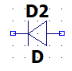
\includegraphics[width=0.45\linewidth]{in0.png}
        \captionsetup{skip=0pt}
        \caption{Вид цепи ограничения: схема 1}
        \label{fig:in0}
    \end{subfigure}
    \hfill
    \begin{subfigure}[b]{0.45\textwidth}
        \centering
        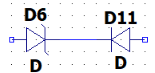
\includegraphics[width=0.9\linewidth]{in00.png}
        \captionsetup{skip=0pt}
        \caption{Вид цепи ограничения: схема 2}
        \label{fig:in00}
    \end{subfigure}
\end{figure}
    \subsection{Таблица 2}
    Обозначим $\alpha$ -- двухвходовый компаратор, $\beta$ -- триггер Шмитта, $\gamma$ -- компаратор с окном
    \begin{center}
        \begin{tabular}{ | m{3.2em} | m{3em}| m{3em} | m{3em} | m{3.7em} | m{3.7em}| m{3.7em} | m{3.7em} |}
        \hline
        Обозн.& задан.& $\alpha$& $\alpha$& $\beta$& $\beta$& $\gamma$& $\gamma$\\ 
        \hline
        $U_{\text{пор}},$ В&$U_\text{ОП},$ В& $U_\text{ОП},$ В &$U_\text{Г},$ В&$U_\text{ВТО},$ В &$U_\text{НТО},$ В &$U_\text{ВТО},$ В &$U_\text{НТО},$ В\\ 
        \hline
        $-2$& $2$ & $1$ &$2$ &$5$ &$2$ &$7.5$ &$6.5$\\ 
        \hline
        \end{tabular}
    \end{center}


    \section{Исследование схем ограничения выходного напряжения на ОУ}
    \subsection{Расчет параметров схемы}
    Соберем схему ограничителя выходного напряжения на ОУ. Вид цепи ограничения представлен на рис. \ref{fig:in0}.
    Рассчитаем параметры резисторов $R_1,R_2$ в соответствии с коэффициентом усиления
    $$
    K_U=\dfrac{U_\text{вых}}{U_\text{вх}}=\dfrac{R_2}{R_1}=2\Rightarrow R_2=2\text{ кОм},\ R_1=1\text{ кОм};
    $$


    \subsection{Схема ограничителя выходного напряжения на ОУ: вид ограничения 1}
    Построим схему в соответствии с вариантом и расчетами. Вид цепи ограничения представлен на рис. \ref{fig:in0}.
    Схема представлена на рис. \ref{fig:scheme1}
    \begin{figure}[H]
        \centering
        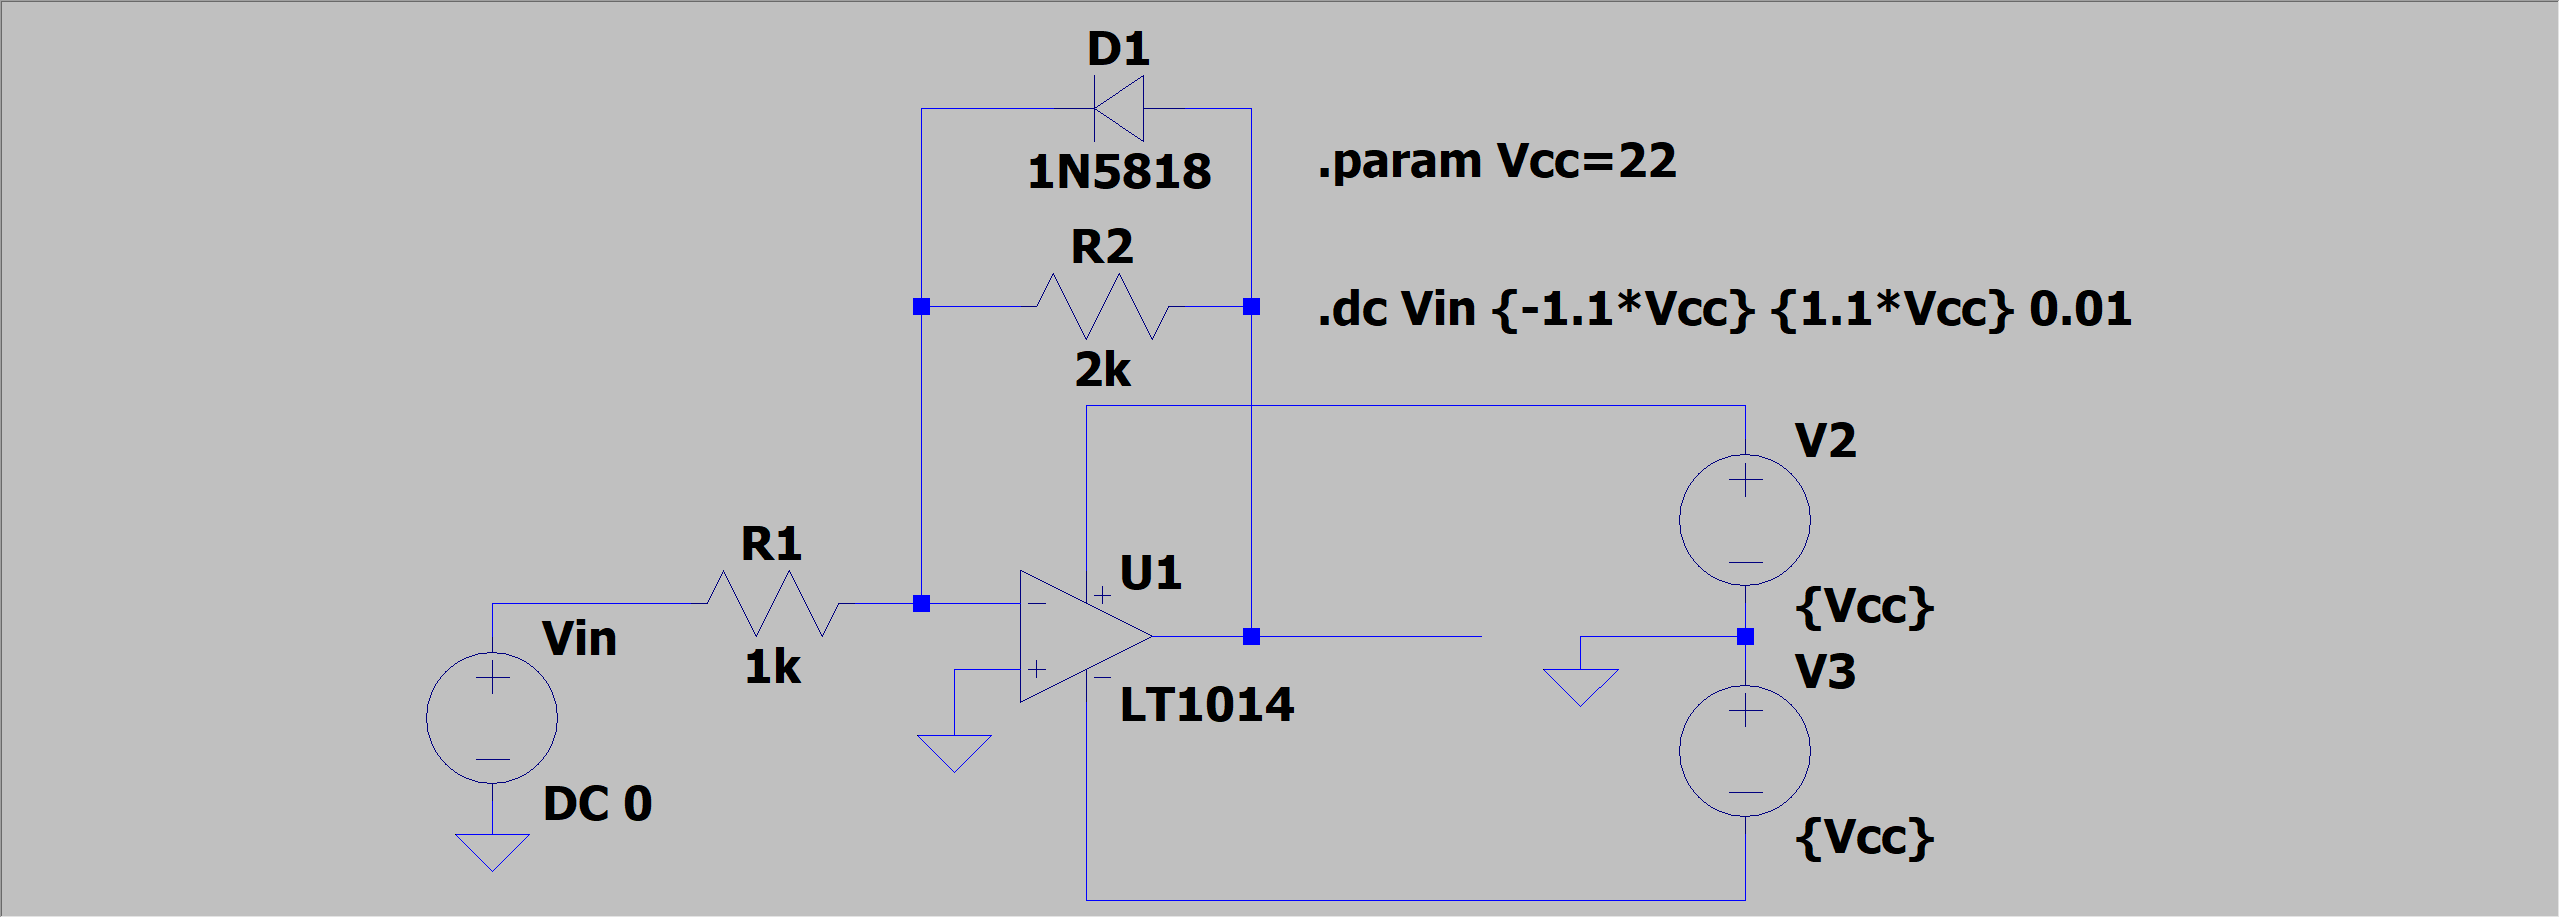
\includegraphics[scale=0.22]{scheme1.png}
        \captionsetup{skip=0pt}
        \caption{Схема ограничителя выходного напряжения на ОУ с видом ограничения 1}
        \label{fig:scheme1}
    \end{figure}


    \subsection{Зависимость выходного напряжения от входного}
    Снимем зависимость $U_\text{вых}=f\left( U_\text{вх} \right)$.
    Значение входного напряжения изменяем в диапазоне от $-1.1U_\text{пит}$ до $1.1U_\text{пит}$.
    Укажем на схеме в LTspice в источник тока Vin значение DC 0 и поставим на схему
    .dc Vin \{-1.1*Vcc\} \{1.1*Vcc\} 0.01. Получаем
    \begin{figure}[H]
        \centering
        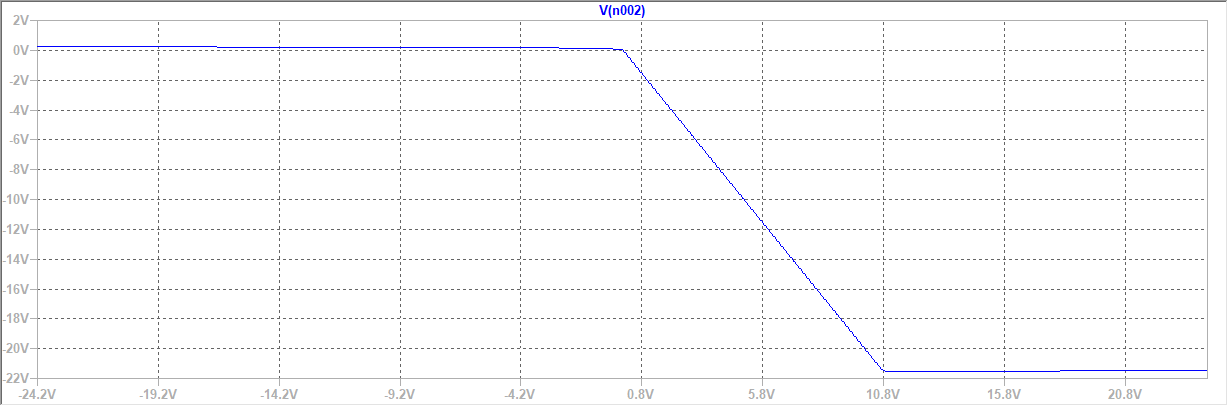
\includegraphics[scale=0.46]{1task_fuin.png}
        \captionsetup{skip=0pt}
        \caption{Выходное напряжение при $-1.1U_\text{пит}\leq U_\text{вх}\leq 1.1U_\text{пит}$ В}
        \label{fig:1task_fuin}
    \end{figure}
    Наблюдаем ограничение для $U_\text{вых}>0$. Для $U_\text{вых}<0$ ограничение по питанию.


    \subsection{Различные входные сигналы}
    Подадим на вход ограничителя от внешнего генератора синусоидальный
    сигнал амплитуды 5 В и частоты 1 кГц SINE(0 5 1k) (амплитуда превышает значение ограничения).
    Зарисуем осциллограмму $U_\text{вых}$
    \begin{figure}[H]
        \centering
        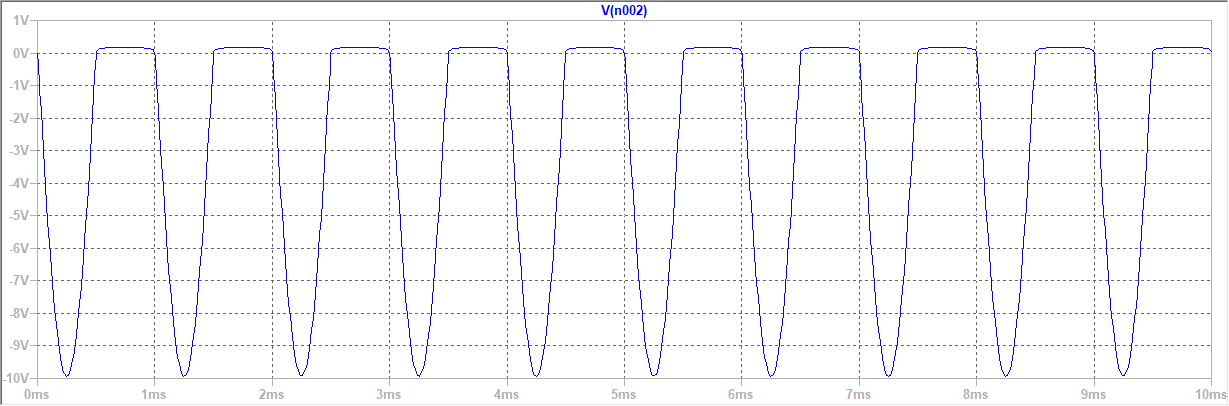
\includegraphics[scale=0.46]{1task_sine_a5_f1k.png}
        \captionsetup{skip=0pt}
        \caption{Выходное напряжение при SINE(0 5 1k)}
        \label{fig:1task_sine_a5_f1k}
    \end{figure}
    \noindent Наблюдаем ограничение для $U_\text{вых}>0$. Попробуем подать постоянный ток в $-5$ В
    \begin{figure}[H]
        \centering
        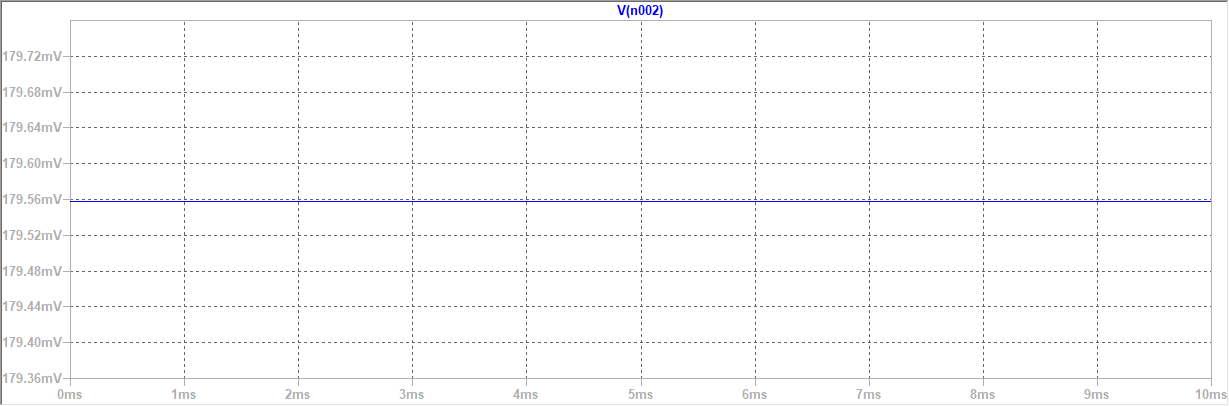
\includegraphics[scale=0.46]{1task_const_m5.png}
        \captionsetup{skip=0pt}
        \caption{Выходное напряжение при постоянном токе $-5$ В}
        \label{fig:1task_const_m5}
    \end{figure}
    \noindent Наблюдаем ограничение для $U_\text{вых}>0$. Попробуем подать $5$ В
    \begin{figure}[H]
        \centering
        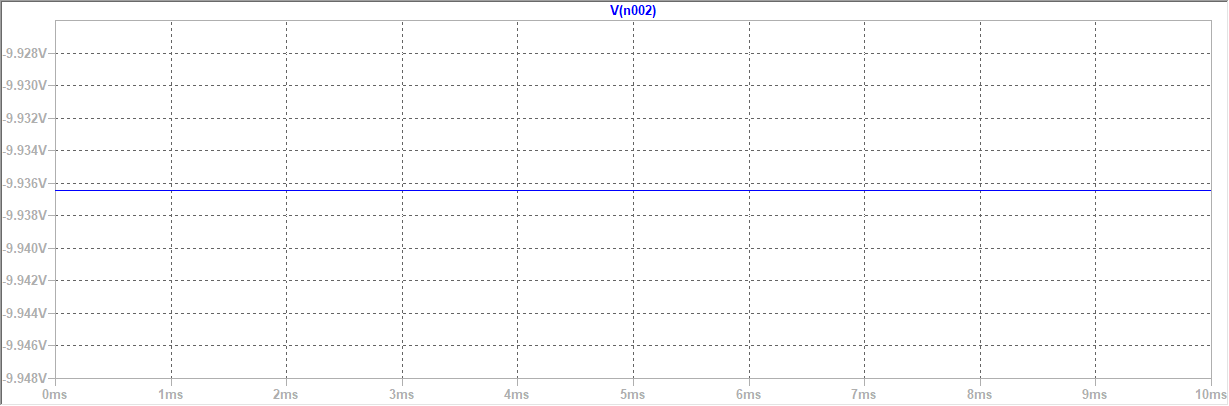
\includegraphics[scale=0.46]{1task_const_5.png}
        \captionsetup{skip=0pt}
        \caption{Выходное напряжение при постоянном токе $5$ В}
        \label{fig:1task_const_5}
    \end{figure}
    \noindent Получилось усиление с коэффициентом $-2$ (инвертирующий усилитель).


    \subsection{Схема ограничителя выходного напряжения на ОУ: вид ограничения 2}
    Поменяем в схеме на рис. \ref{fig:scheme1} вид ограничения на представленный на рис. \ref{fig:in00}.
    Обновленная схема представлена на рис. \ref{fig:scheme3}
    \begin{figure}[H]
        \centering
        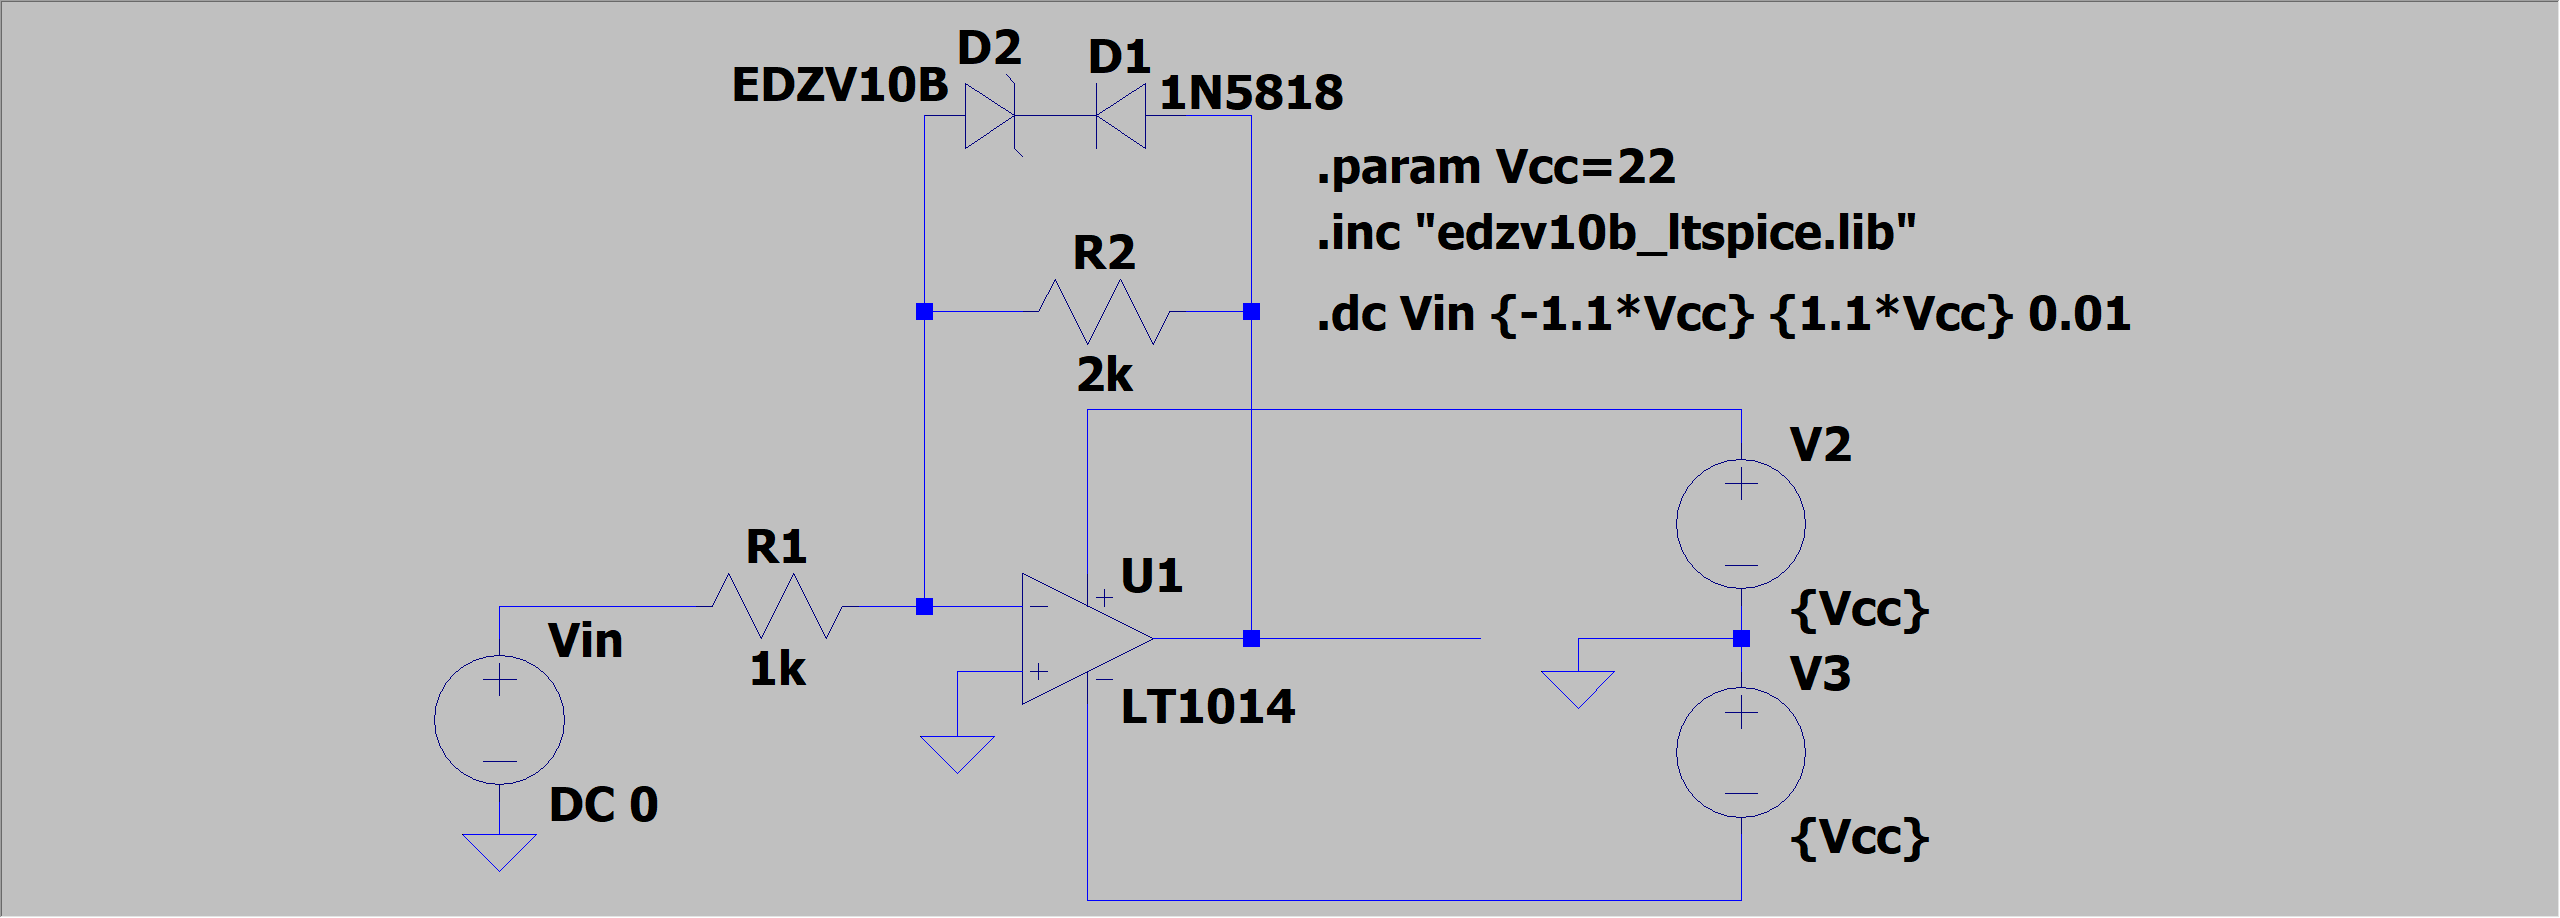
\includegraphics[scale=0.22]{scheme3.png}
        \captionsetup{skip=0pt}
        \caption{Схема ограничителя выходного напряжения на ОУ с видом ограничения 2}
        \label{fig:scheme3}
    \end{figure}


    \subsection{Зависимость выходного напряжения от входного}
    Снимем зависимость $U_\text{вых}=f\left( U_\text{вх} \right)$ аналогичным образом.
    Получаем
    \begin{figure}[H]
        \centering
        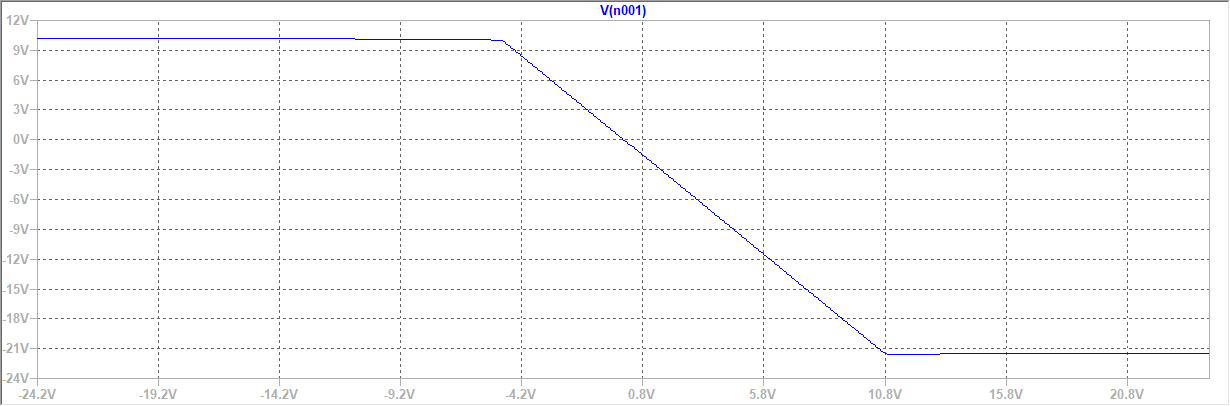
\includegraphics[scale=0.46]{1task2_fuin.png}
        \captionsetup{skip=0pt}
        \caption{Выходное напряжение при $-1.1U_\text{пит}\leq U_\text{вх}\leq 1.1U_\text{пит}$ В}
        \label{fig:1task2_fuin}
    \end{figure}
    Наблюдаем ограничение для $U_\text{вых}>10$. Для $U_\text{вых}<0$ ограничение по питанию.


    \subsection{Различные входные сигналы}
    Проведем аналогичный первому виду ограничения эксперимент.
    Зарисуем осциллограмму $U_\text{вых}$
    \begin{figure}[H]
        \centering
        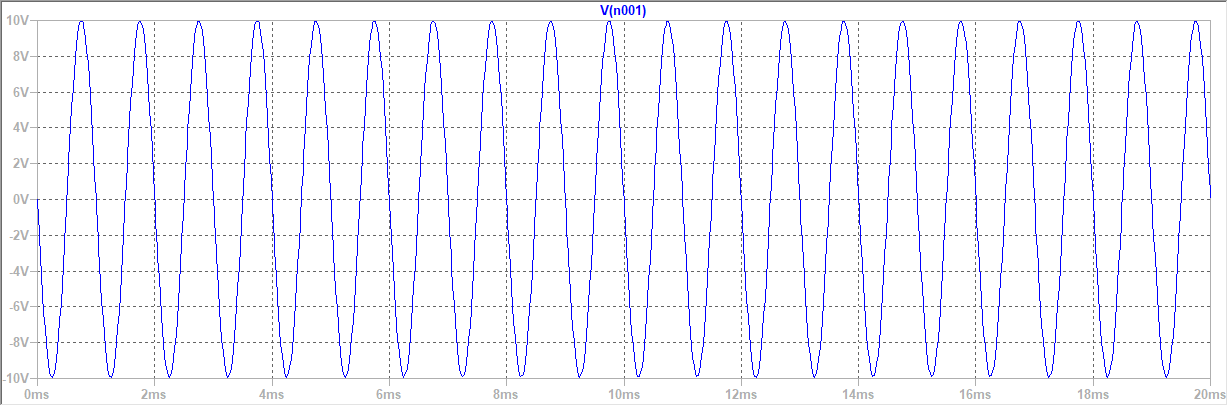
\includegraphics[scale=0.46]{1task2_sine_a5_f1k.png}
        \captionsetup{skip=0pt}
        \caption{Выходное напряжение при SINE(0 5 1k)}
        \label{fig:1task2_sine_a5_f1k}
    \end{figure}
    \noindent Теперь ограничение для $U_\text{вых}>10$ -- видим целую синусоиду. Попробуем подать постоянный ток в $-5$ В
    \begin{figure}[H]
        \centering
        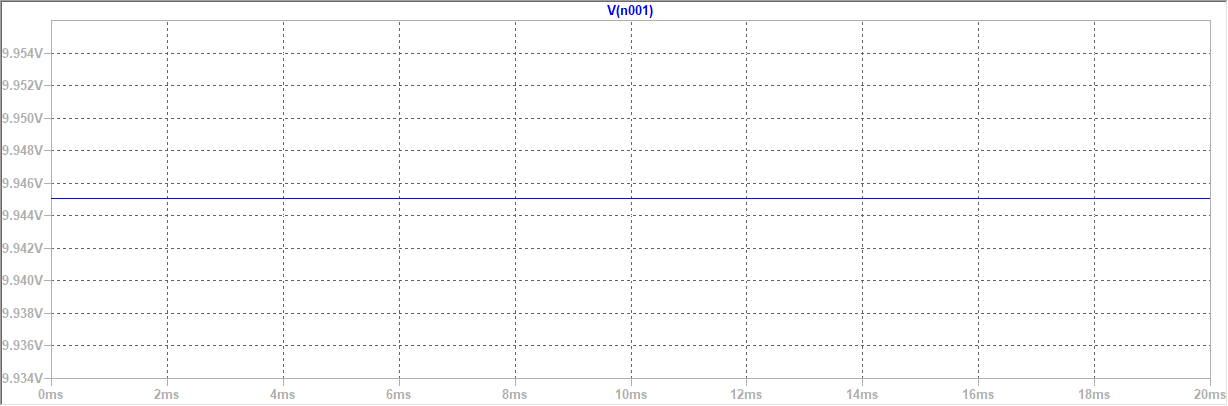
\includegraphics[scale=0.46]{1task2_const_m5.png}
        \captionsetup{skip=0pt}
        \caption{Выходное напряжение при постоянном токе $-5$ В}
        \label{fig:1task2_const_m5}
    \end{figure}
    \noindent Получилось усиление с коэффициентом $-2$. Попробуем подать $5$ В
    \begin{figure}[H]
        \centering
        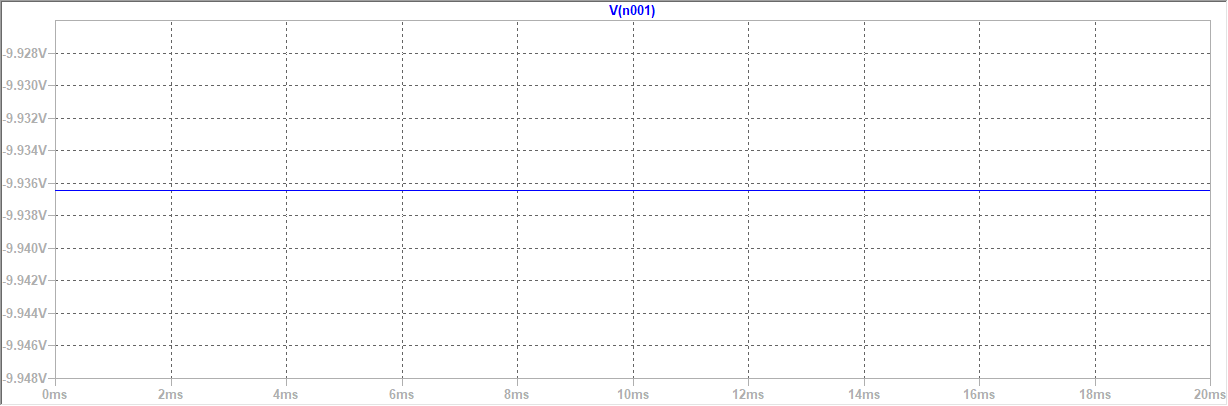
\includegraphics[scale=0.46]{1task2_const_5.png}
        \captionsetup{skip=0pt}
        \caption{Выходное напряжение при постоянном токе $5$ В}
        \label{fig:1task2_const_5}
    \end{figure}
    \noindent Получилось усиление с коэффициентом $-2$.


    \subsection{Вывод относительно влияния нелинейных элементов в цепи обратной связи}
    При использовании только диода выходное напряжение ограничивалось на уровне чуть больше нуля
    (порог открывания диода). Добавление стабилитрона внесло сдвиг порога ограничения. Сигнал
    стал ограничиваться на уровне около 10 В (напряжение стабилизации 10 В). Таким образом,
    нелинейные элементы в цепи ОС позволяют формировать управляемое ограничение.


    \section{Исследование нуль-компаратора}
    \subsection{Схема нуль-компаратора}
    Соберем схему нуль-компаратора на ОУ. Установим
    значение сопротивления $R_1=10$ кОм. Схема
    представлена на рис. \ref{fig:scheme5}
    \begin{figure}[H]
        \centering
        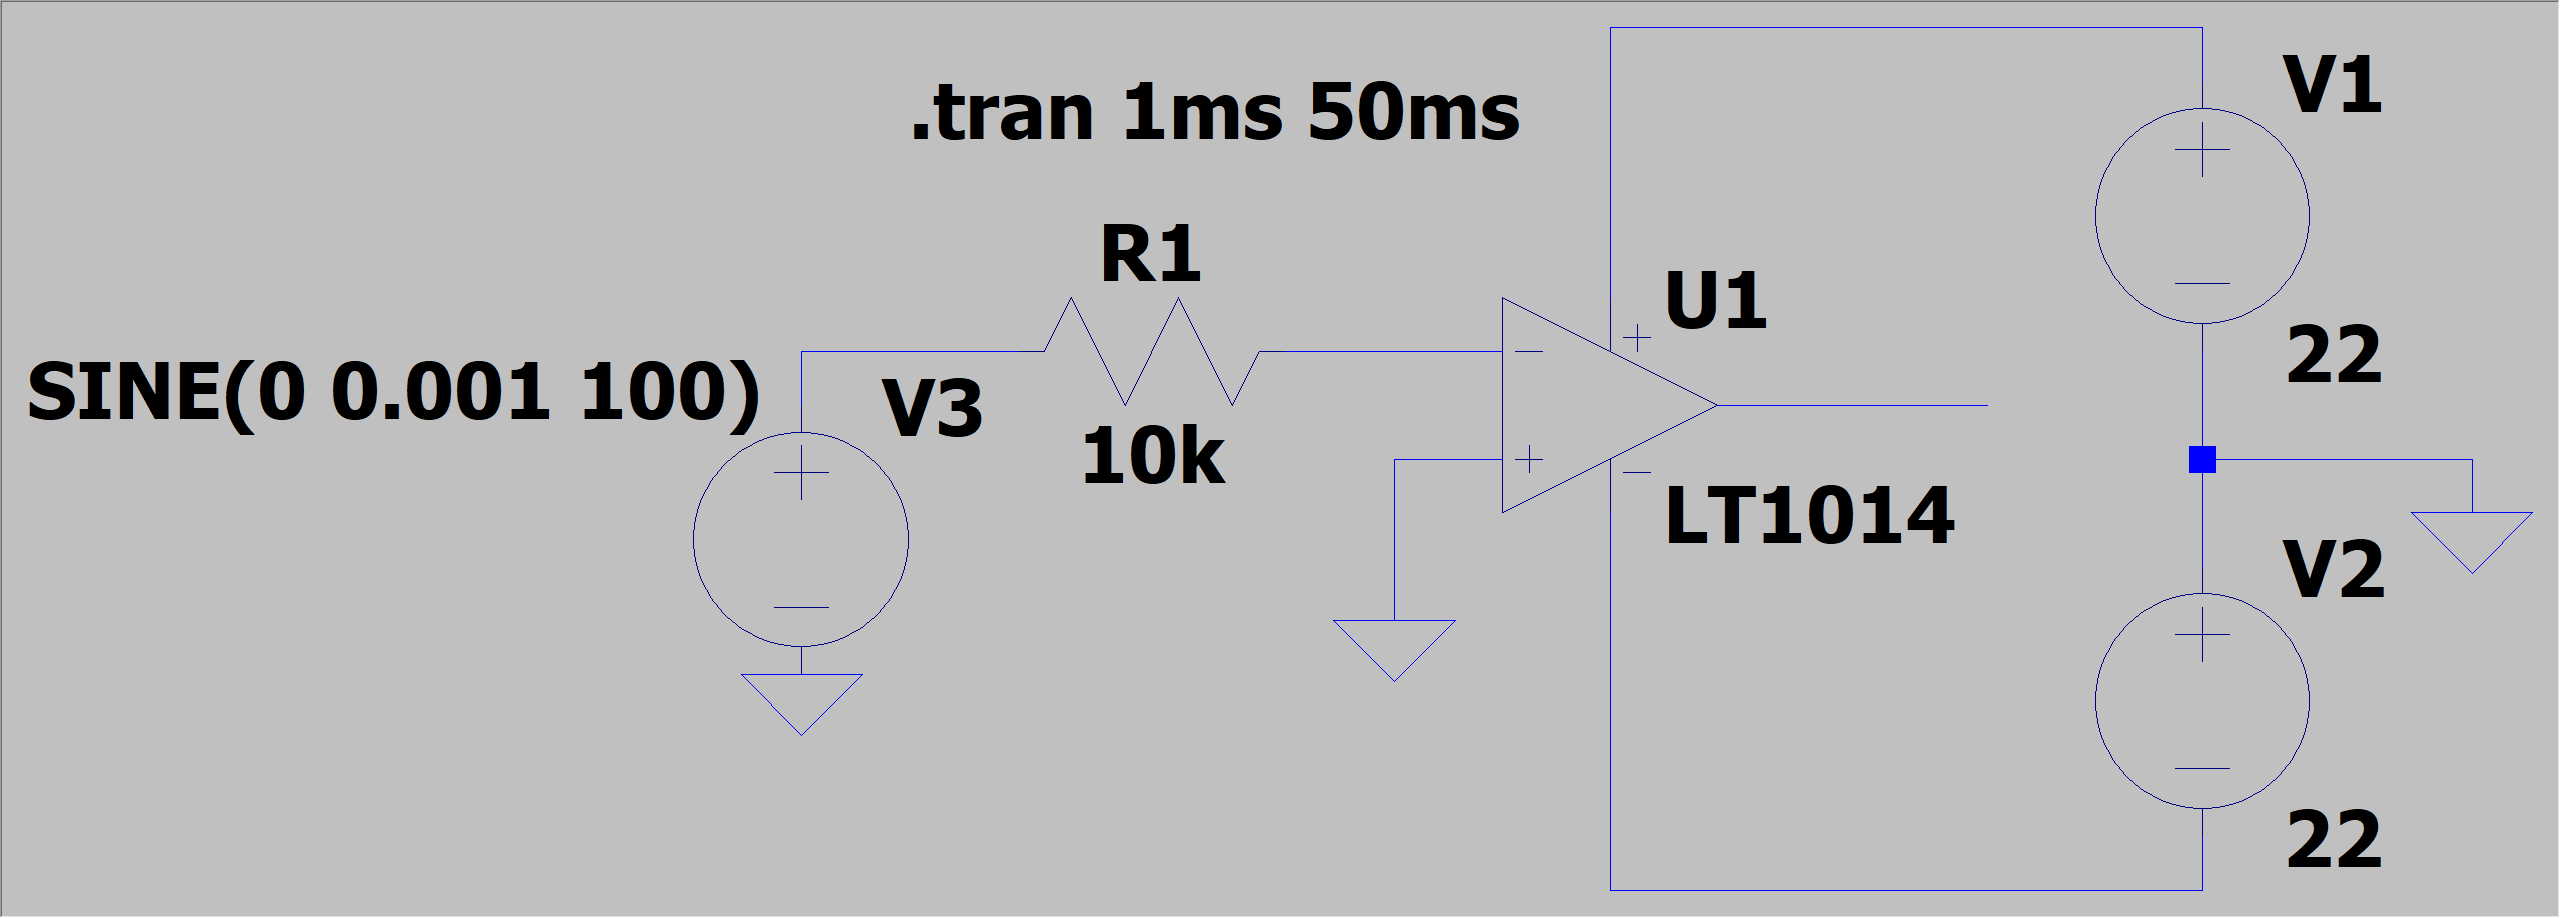
\includegraphics[scale=0.22]{scheme5.png}
        \captionsetup{skip=0pt}
        \caption{Схема нуль-компаратора}
        \label{fig:scheme5}
    \end{figure}


    \subsection{Исследование синусоидального сигнала}
    Подадим на вход системы синусоидальный сигнал с амплитудой 1 мВ,
    частоту будем варьировать $f=0.1,0.3,0.5,1$ кГц. Снимем осцилограммы
    $U_\text{вх}$ и $U_\text{вых}$. После этого изменим амплитуду синусоиды на 1 В и повторим эксперимент
    \begin{figure}[H]
        \centering
        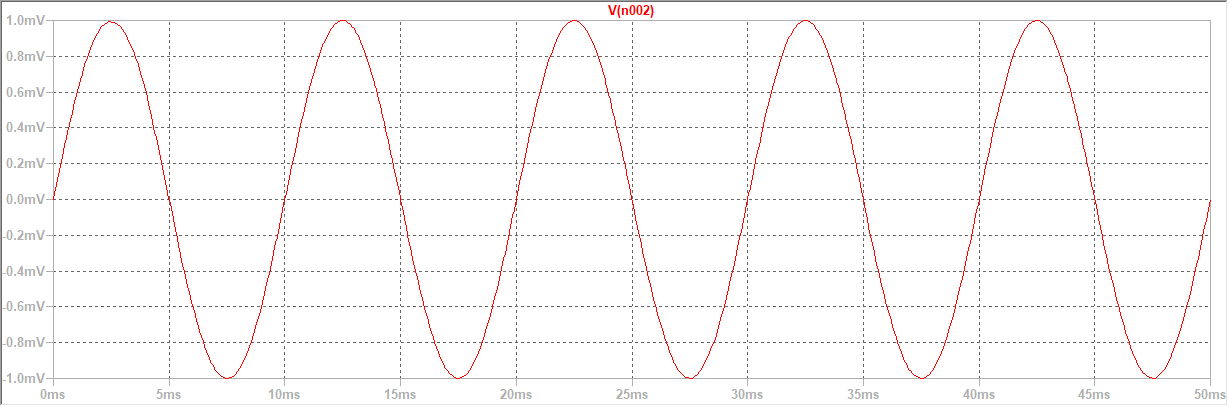
\includegraphics[scale=0.46]{3task_sine_in_1mV_100f.png}
        \captionsetup{skip=0pt}
        \caption{Входное напряжение при SINE(0 0.001 100)}
        \label{fig:3task_sine_in_1mV_100f}
    \end{figure}
    \begin{figure}[H]
        \centering
        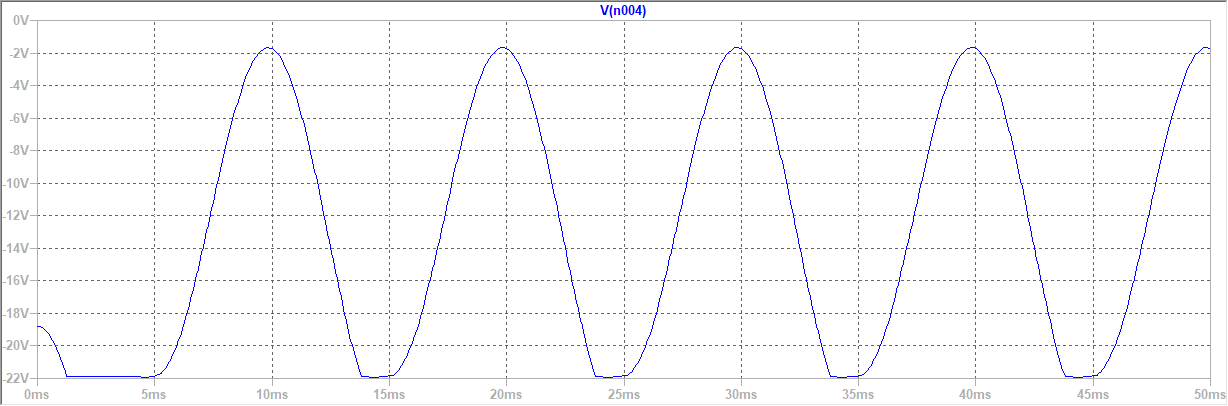
\includegraphics[scale=0.46]{3task_sine_out_1mV_100f.png}
        \captionsetup{skip=0pt}
        \caption{Выходное напряжение при SINE(0 0.001 100)}
        \label{fig:3task_sine_out_1mV_100f}
    \end{figure}
    \begin{figure}[H]
        \centering
        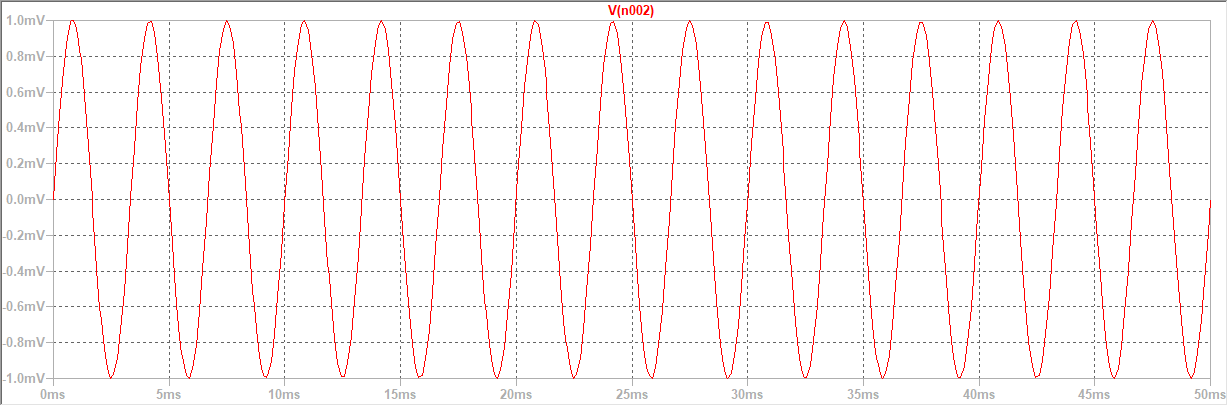
\includegraphics[scale=0.46]{3task_sine_in_1mV_300f.png}
        \captionsetup{skip=0pt}
        \caption{Входное напряжение при SINE(0 0.001 300)}
        \label{fig:3task_sine_in_1mV_300f}
    \end{figure}
    \begin{figure}[H]
        \centering
        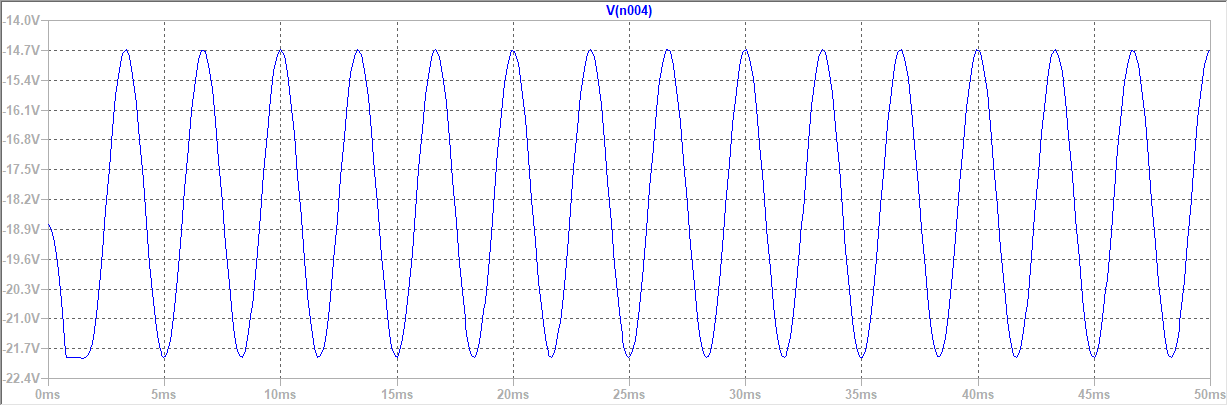
\includegraphics[scale=0.46]{3task_sine_out_1mV_300f.png}
        \captionsetup{skip=0pt}
        \caption{Выходное напряжение при SINE(0 0.001 300)}
        \label{fig:3task_sine_out_1mV_300f}
    \end{figure}
    \begin{figure}[H]
        \centering
        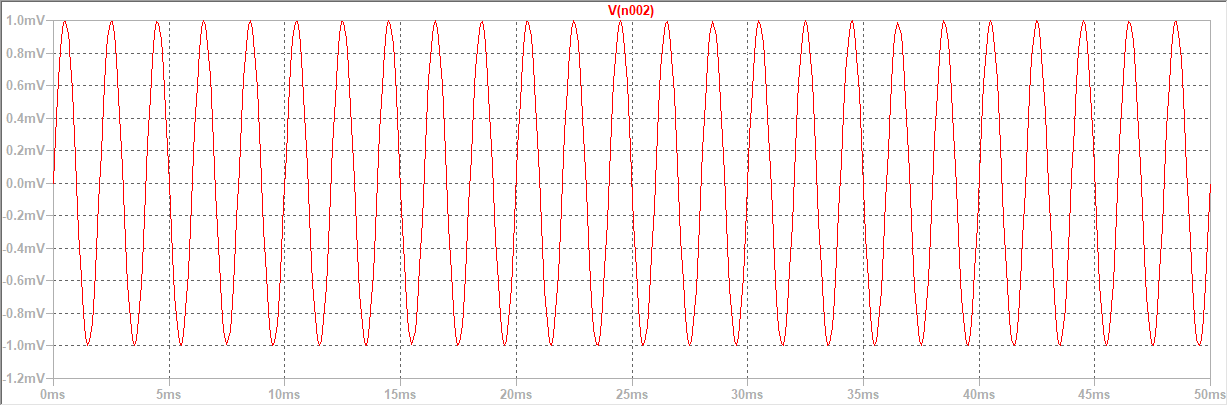
\includegraphics[scale=0.46]{3task_sine_in_1mV_500f.png}
        \captionsetup{skip=0pt}
        \caption{Входное напряжение при SINE(0 0.001 500)}
        \label{fig:3task_sine_in_1mV_500f}
    \end{figure}
    \begin{figure}[H]
        \centering
        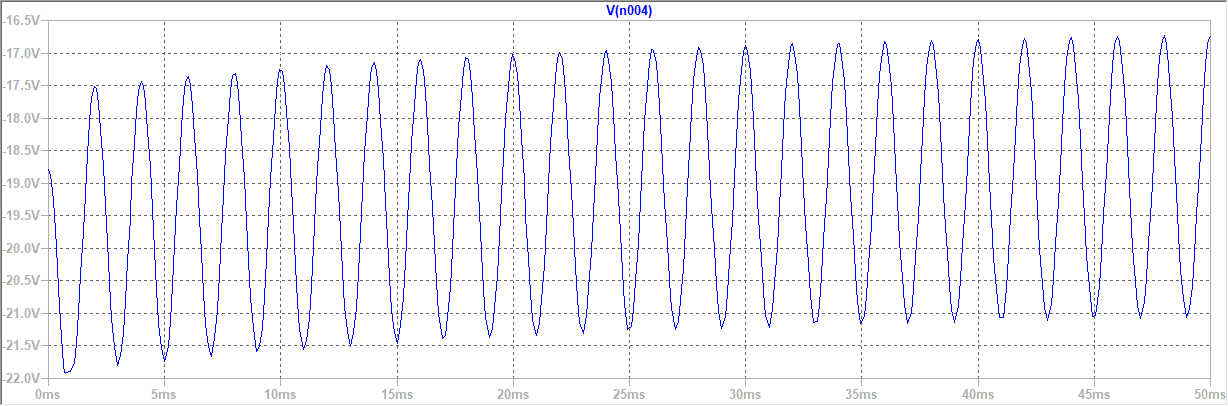
\includegraphics[scale=0.46]{3task_sine_out_1mV_500f.png}
        \captionsetup{skip=0pt}
        \caption{Выходное напряжение при SINE(0 0.001 500)}
        \label{fig:3task_sine_out_1mV_500f}
    \end{figure}
    \begin{figure}[H]
        \centering
        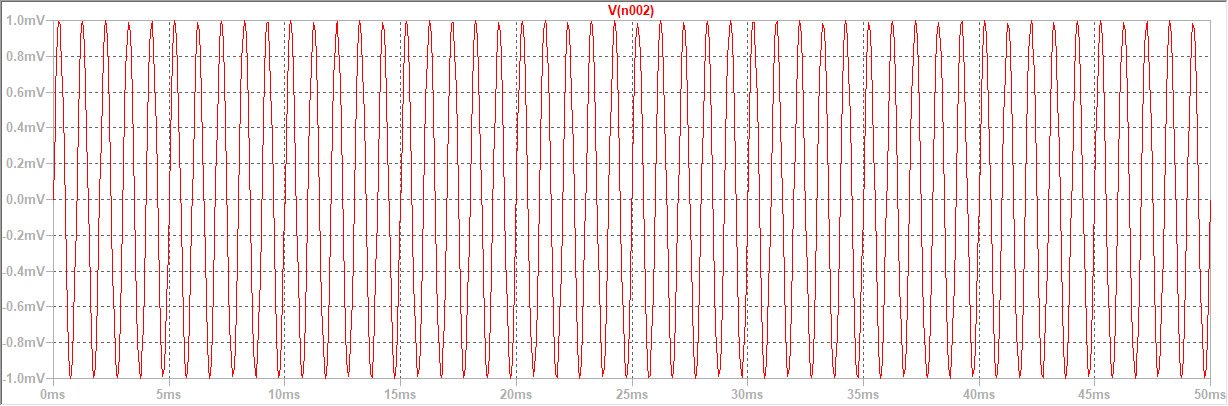
\includegraphics[scale=0.46]{3task_sine_in_1mV_1kf.png}
        \captionsetup{skip=0pt}
        \caption{Входное напряжение при SINE(0 0.001 1k)}
        \label{fig:3task_sine_in_1mV_1kf}
    \end{figure}
    \begin{figure}[H]
        \centering
        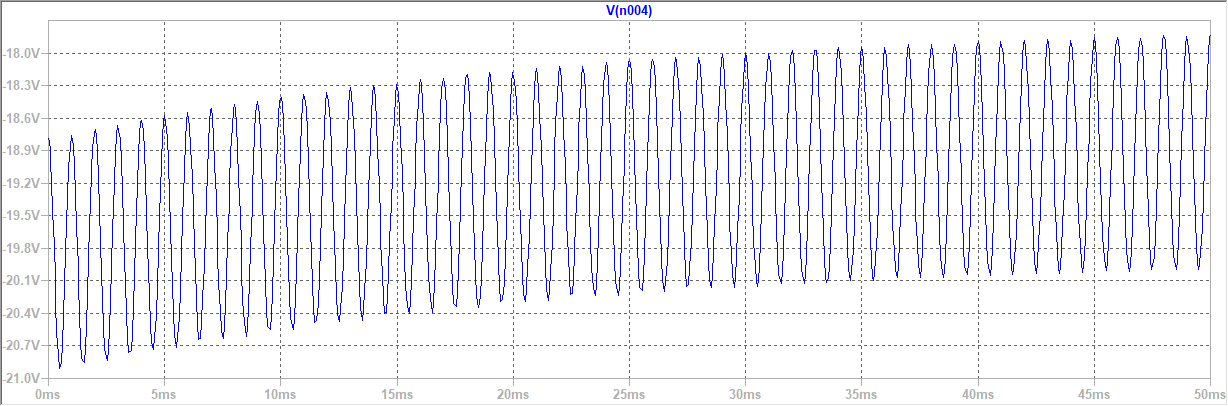
\includegraphics[scale=0.46]{3task_sine_out_1mV_1kf.png}
        \captionsetup{skip=0pt}
        \caption{Выходное напряжение при SINE(0 0.001 1k)}
        \label{fig:3task_sine_out_1mV_1kf}
    \end{figure}
    \begin{figure}[H]
        \centering
        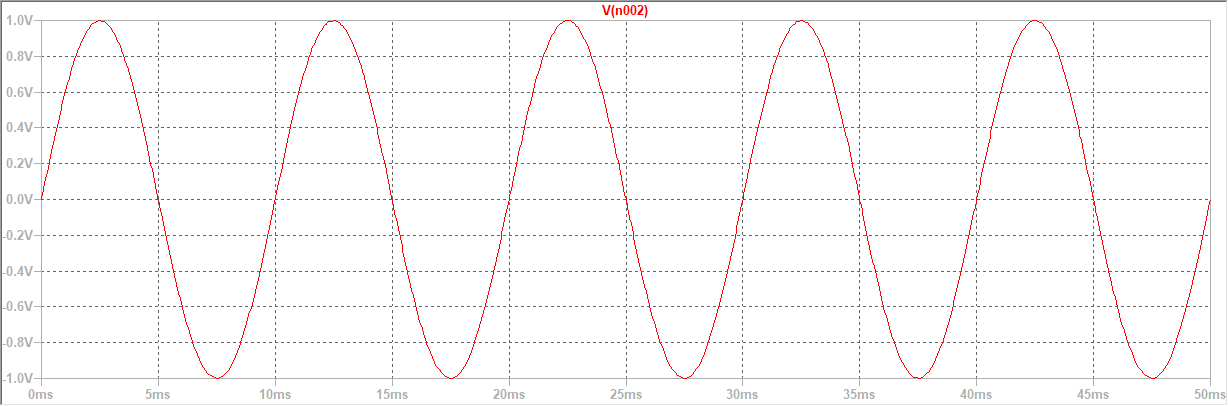
\includegraphics[scale=0.46]{3task_sine_in_1V_100f.png}
        \captionsetup{skip=0pt}
        \caption{Входное напряжение при SINE(0 1 100)}
        \label{fig:3task_sine_in_1V_100f}
    \end{figure}
    \begin{figure}[H]
        \centering
        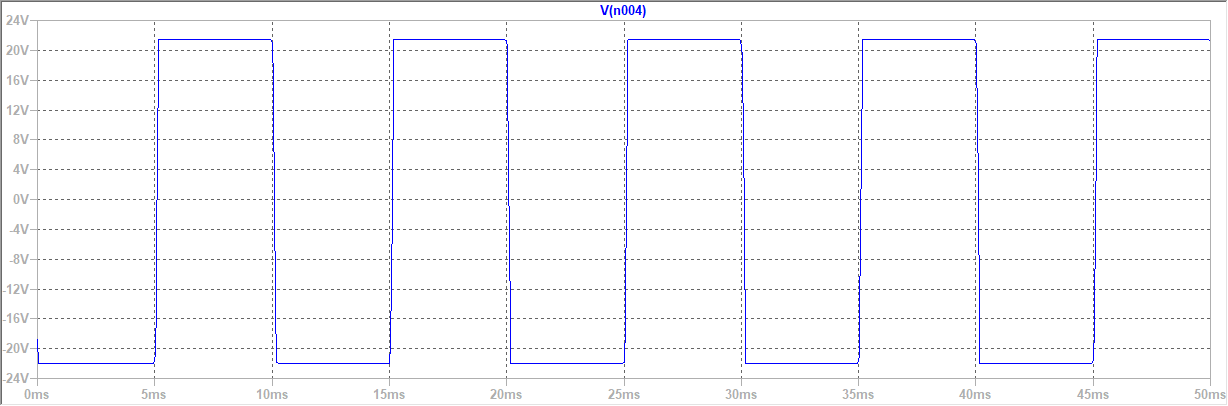
\includegraphics[scale=0.46]{3task_sine_out_1V_100f.png}
        \captionsetup{skip=0pt}
        \caption{Выходное напряжение при SINE(0 1 100)}
        \label{fig:3task_sine_out_1V_100f}
    \end{figure}
    \begin{figure}[H]
        \centering
        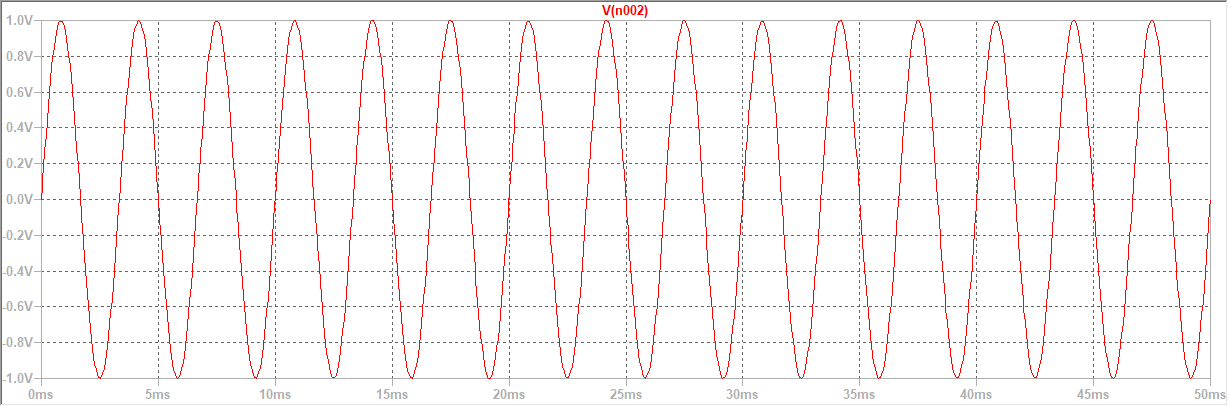
\includegraphics[scale=0.46]{3task_sine_in_1V_300f.png}
        \captionsetup{skip=0pt}
        \caption{Входное напряжение при SINE(0 1 300)}
        \label{fig:3task_sine_in_1V_300f}
    \end{figure}
    \begin{figure}[H]
        \centering
        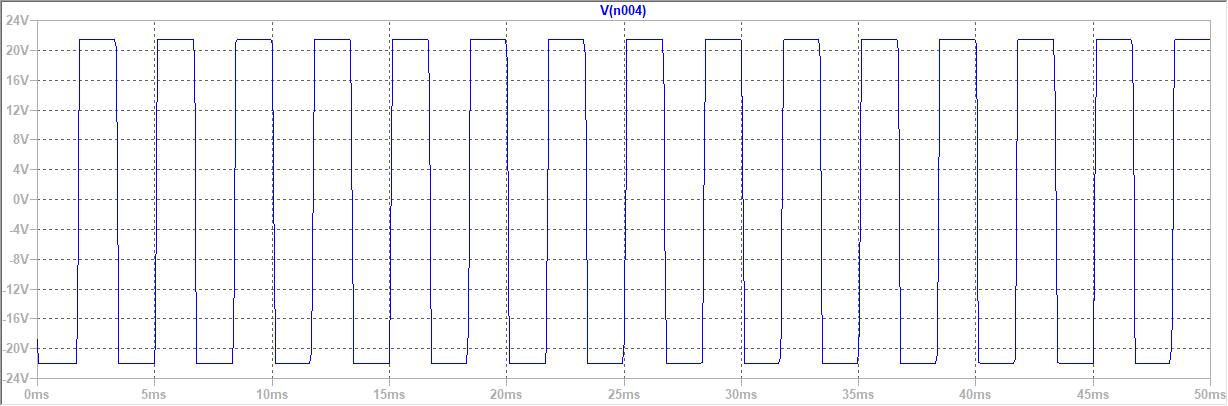
\includegraphics[scale=0.46]{3task_sine_out_1V_300f.png}
        \captionsetup{skip=0pt}
        \caption{Выходное напряжение при SINE(0 1 300)}
        \label{fig:3task_sine_out_1V_300f}
    \end{figure}
    \begin{figure}[H]
        \centering
        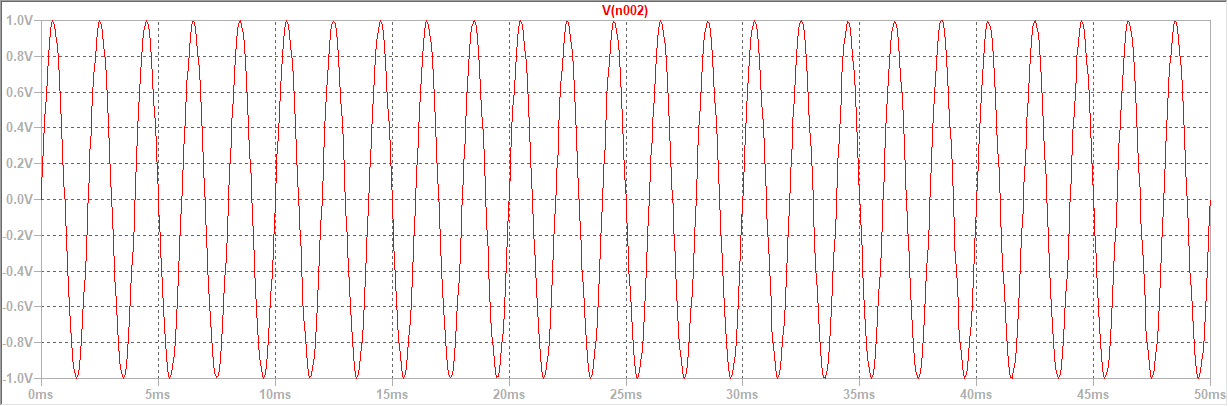
\includegraphics[scale=0.46]{3task_sine_in_1V_500f.png}
        \captionsetup{skip=0pt}
        \caption{Входное напряжение при SINE(0 1 500)}
        \label{fig:3task_sine_in_1V_500f}
    \end{figure}
    \begin{figure}[H]
        \centering
        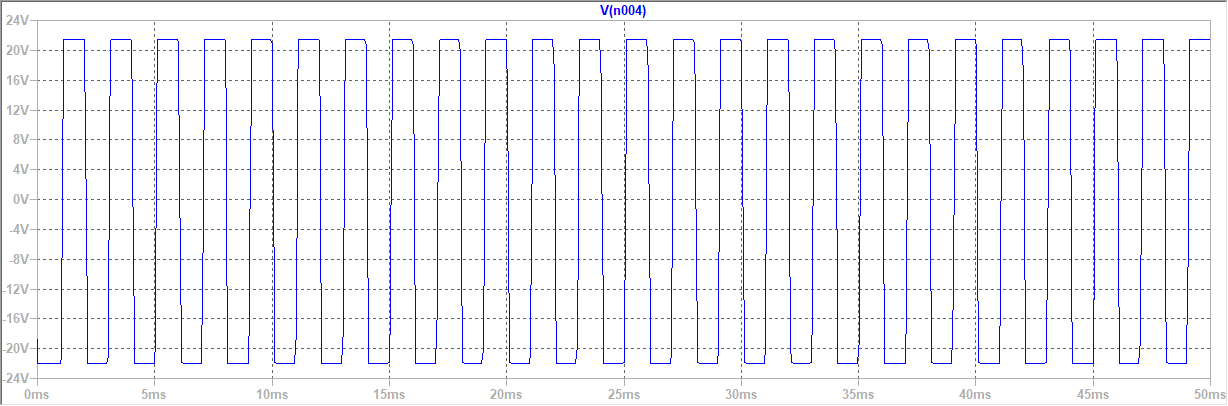
\includegraphics[scale=0.46]{3task_sine_out_1V_500f.png}
        \captionsetup{skip=0pt}
        \caption{Выходное напряжение при SINE(0 1 500)}
        \label{fig:3task_sine_out_1V_500f}
    \end{figure}
    \begin{figure}[H]
        \centering
        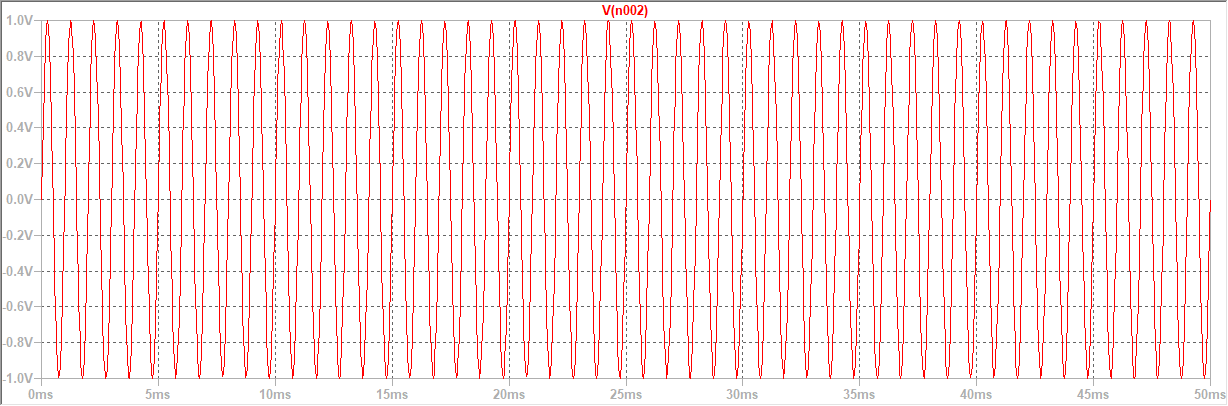
\includegraphics[scale=0.46]{3task_sine_in_1V_1kf.png}
        \captionsetup{skip=0pt}
        \caption{Входное напряжение при SINE(0 1 1k)}
        \label{fig:3task_sine_in_1V_1kf}
    \end{figure}
    \begin{figure}[H]
        \centering
        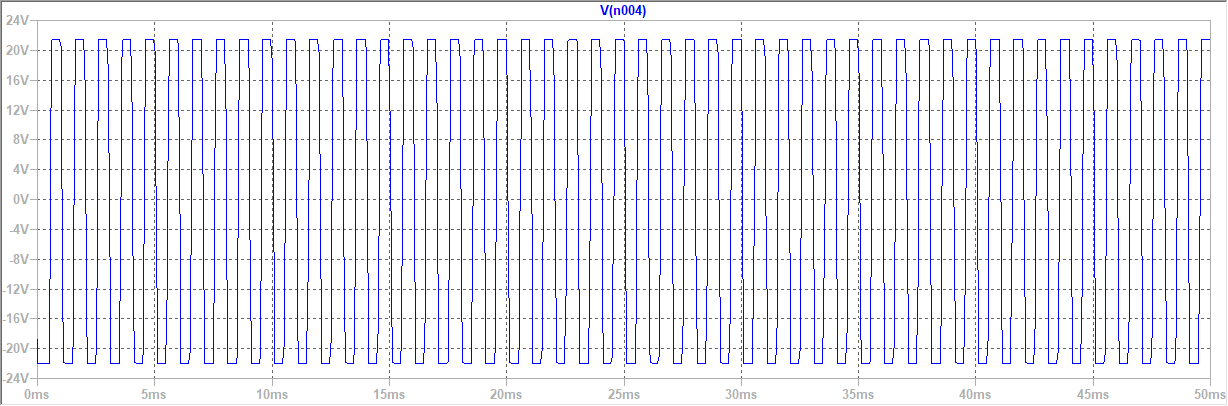
\includegraphics[scale=0.46]{3task_sine_out_1V_1kf.png}
        \captionsetup{skip=0pt}
        \caption{Выходное напряжение при SINE(0 1 1k)}
        \label{fig:3task_sine_out_1V_1kf}
    \end{figure}


    \subsection{Вывод}
    Уровня входного сигнала в 1 мВ недостаточно для корректной работы компаратора.
    При усилении сигнала до 1 В компаратор работает стабильно и верно.


    \section{Исследование одновходового компаратора}
    \subsection{Расчет параметров схемы}
    Соберем схему одновходового компаратора.
    Зададим значение сопротивления резистора $R_1=100$ Ом.
    Из таблицы 2 берем значение $U_\text{пор}=-2$ В. По условию $U_\text{ОП}=10$ В.
    Рассчитаем значения сопротивлений резисторов $R_2,R_3$
    $$
    U_\text{пор}=-U_\text{ОП}\dfrac{R_1}{R_2},\ R_3=\dfrac{R_1R_2}{R_1+R_2},
    $$
    $$
    -2=-10\cdot\dfrac{100}{R_2}\Rightarrow R_2=500\text{ Ом},\ R_3=\dfrac{100\cdot500}{100+500}\approx83.33\text{ Ом};
    $$


    \subsection{Схема одновходового компаратора}
    Соберем схему согласно расчетам и варианту. Схема представлена на рис. \ref{fig:scheme6}
    \begin{figure}[H]
        \centering
        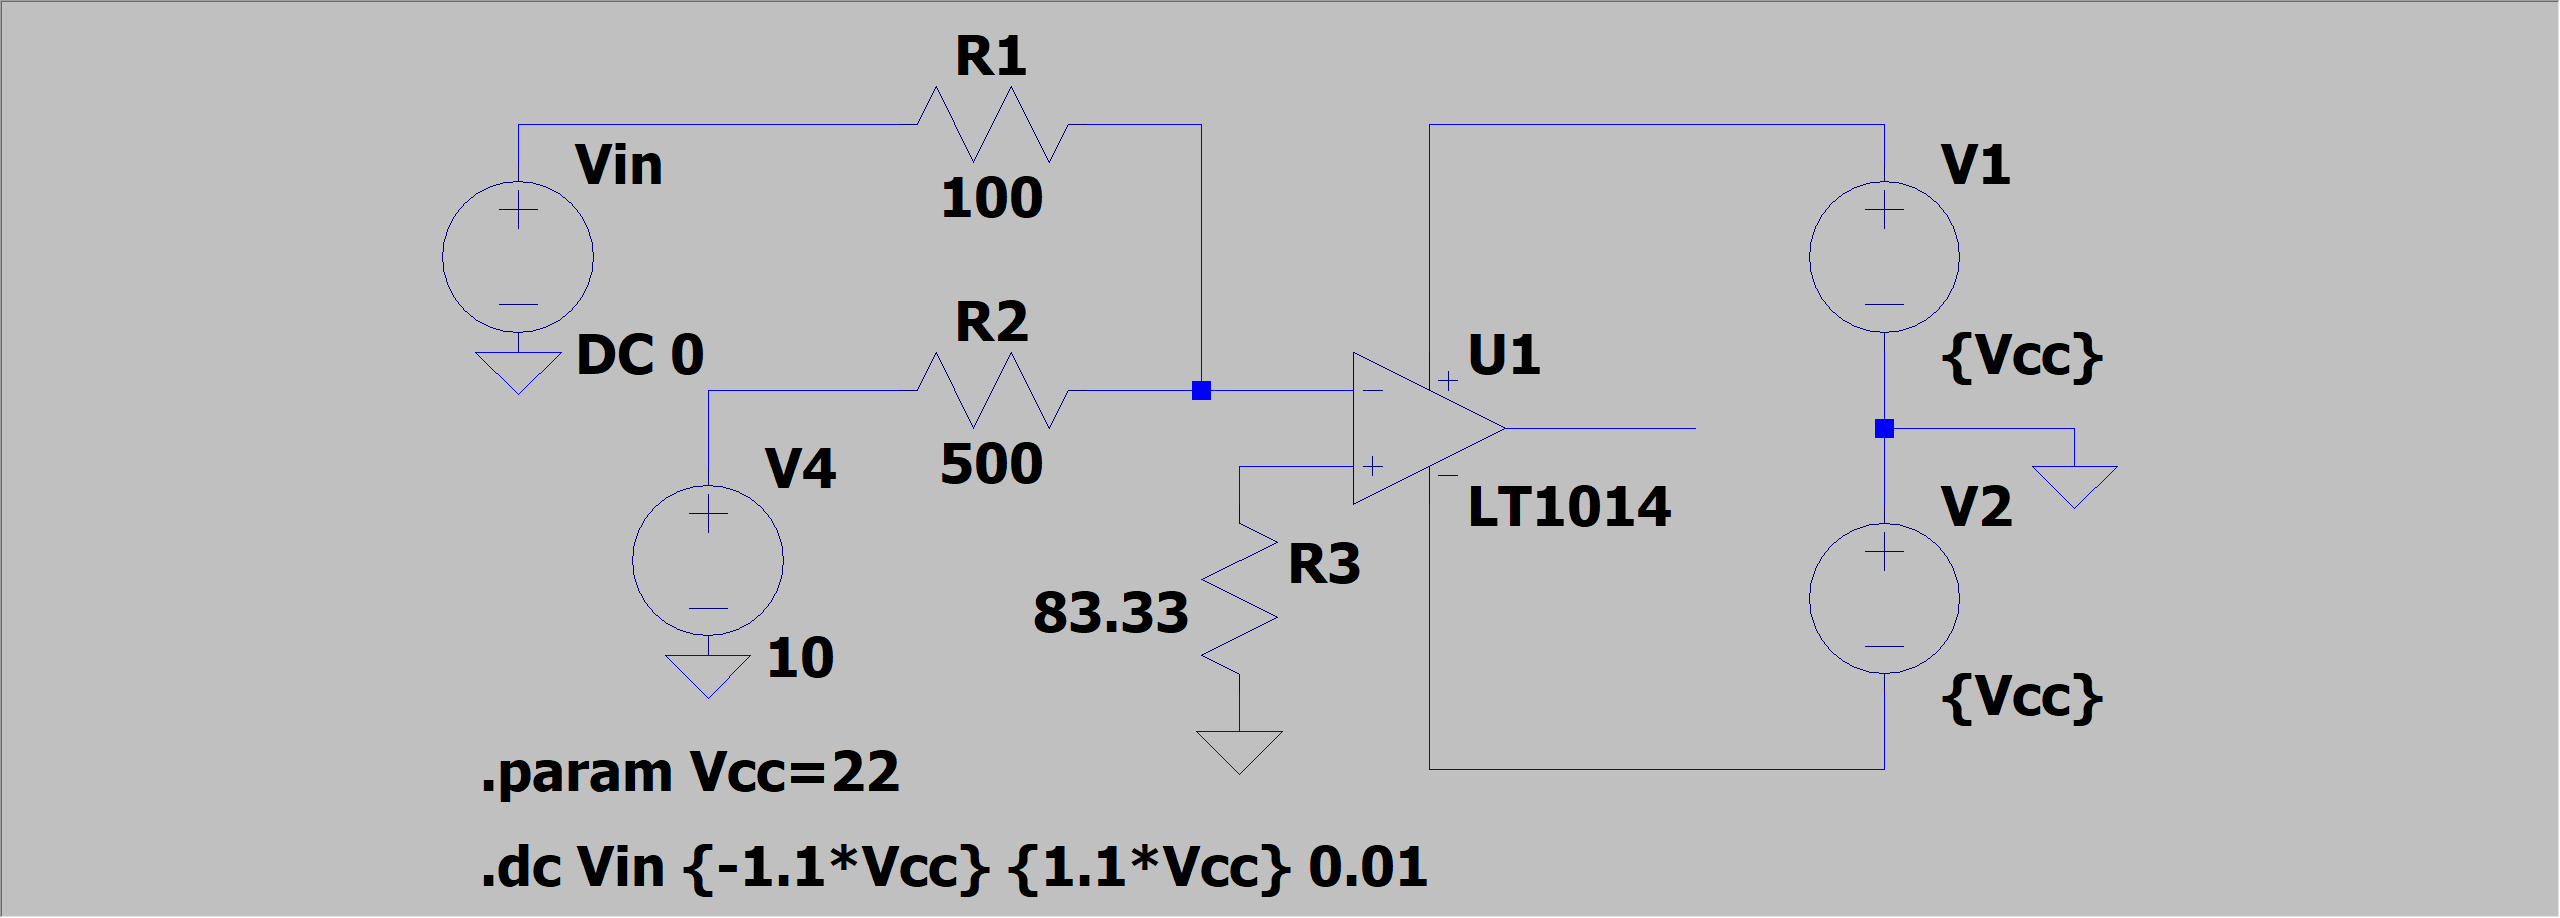
\includegraphics[scale=0.22]{scheme6.png}
        \captionsetup{skip=0pt}
        \caption{Схема одновходового компаратора}
        \label{fig:scheme6}
    \end{figure}

    
    \subsection{Зависимость выходного напряжения от входного}
    Снимем зависимость $U_\text{вых}=f\left( U_\text{вх} \right)$ аналогично
    заданию с ограничителем. Получаем
    \begin{figure}[H]
        \centering
        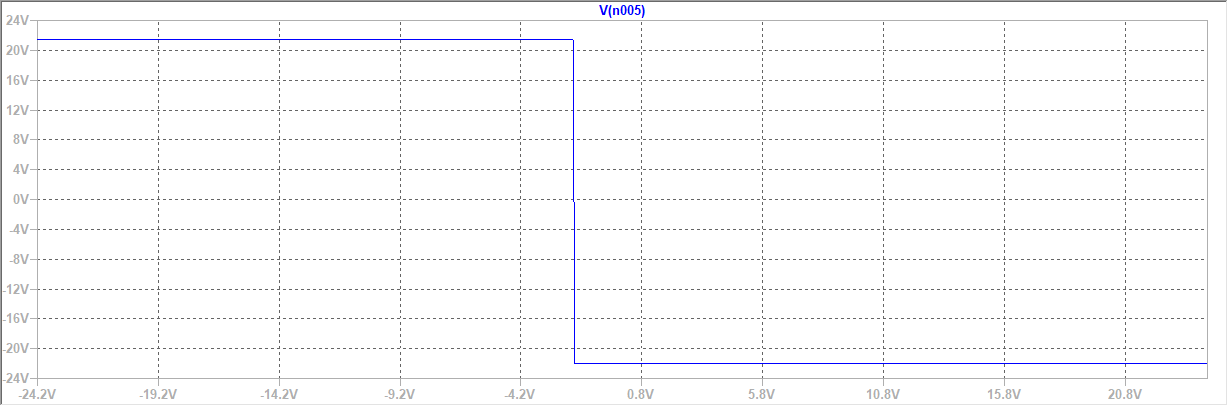
\includegraphics[scale=0.46]{4task_fuin.png}
        \captionsetup{skip=0pt}
        \caption{Выходное напряжение при $-1.1U_\text{пит}\leq U_\text{вх}\leq 1.1U_\text{пит}$ В, $U_\text{пор эксп}=-1.986$ В}
        \label{fig:4task_fuin}
    \end{figure}


    \subsection{Вывод}
    При прохождении сигналом порога в $-2$ В компаратор корректно
    переключился между положительным и отрицательным насыщением.

    
    \section{Исследование двухвходового компаратора}
    \subsection{Схема двухвходового компаратора без гистерезиса}
    Соберем схему двухвходового компаратора без гистерезиса на ОУ при $U_\text{ОП}=1$.
    Значения резисторов произвольные -- они не влияют на порог сравнения.
    Схема представлена на рис. \ref{fig:scheme7}
    \begin{figure}[H]
        \centering
        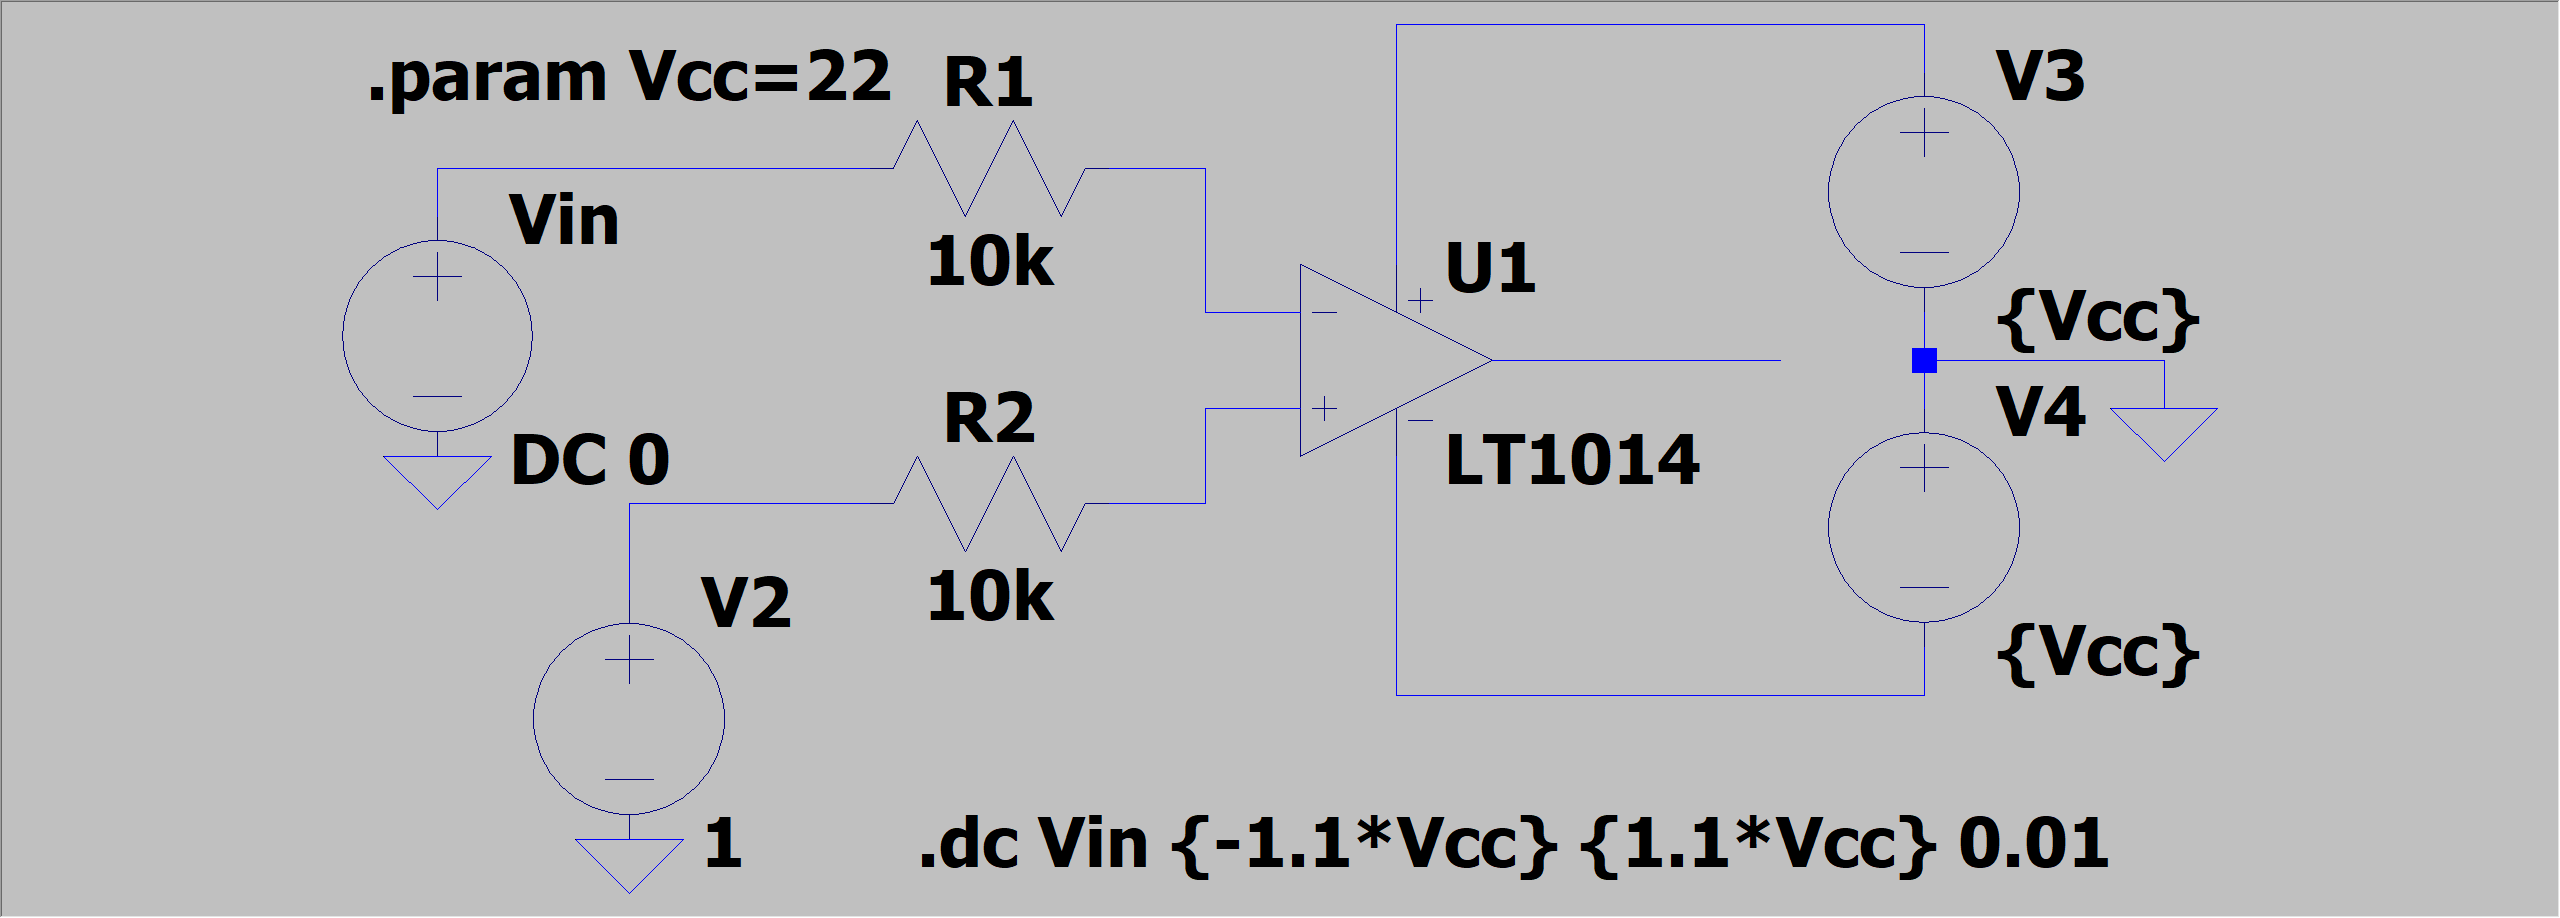
\includegraphics[scale=0.22]{scheme7.png}
        \captionsetup{skip=0pt}
        \caption{Схема двухвходового компаратора без гистерезиса}
        \label{fig:scheme7}
    \end{figure}


    \subsection{Зависимость выходного напряжения от входного}
    Снимем зависимость $U_\text{вых}=f\left( U_\text{вх} \right)$ как в задании с ограничителем.
    Получаем
    \begin{figure}[H]
        \centering
        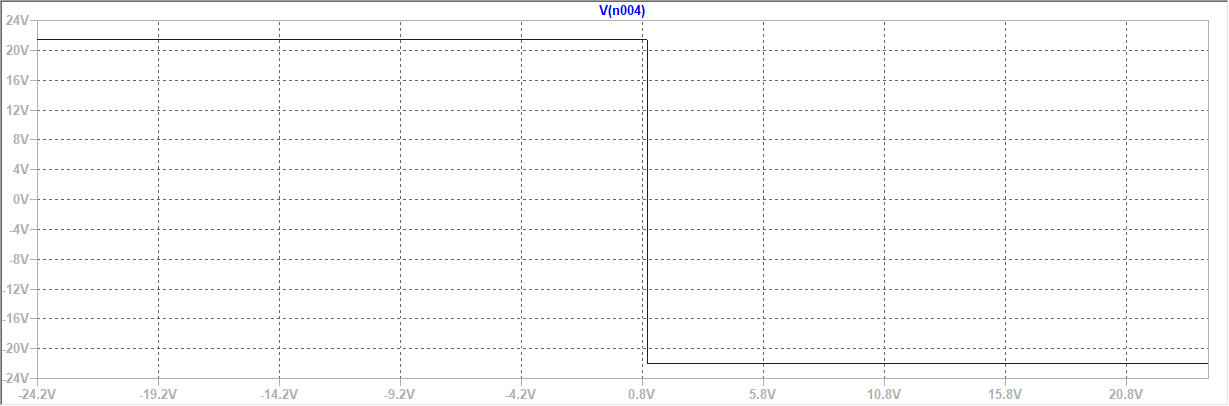
\includegraphics[scale=0.46]{5task_fuin.png}
        \captionsetup{skip=0pt}
        \caption{Выходное напряжение при $-1.1U_\text{пит}\leq U_\text{вх}\leq 1.1U_\text{пит}$ В, $U_\text{пор эксп}=1.014$ В}
        \label{fig:5task_fuin}
    \end{figure}


    \subsection{Вывод}
    Вывод аналогичен заданию с одновходовым компаратором
    -- двухвходовый компаратор без гистерезиса
    отработал корректно.


    \subsection{Расчет параметров схемы двухвходового компаратора с гистерезисом на ОУ}
    Соберем схему двухвходового компаратора с гистерезисом на операционном
    усилителе. Рассчитаем параметры схемы. $R_3$ берем произвольно, он не
    влияет на гистерезис. Зафиксируем $R_2=10\text{ кОм}$. В нашем случае
    $U_\text{пит}=U_{\text{нас}+}=|U_{\text{нас}-}|=22$ В. Из
    таблицы 2 берем значение размаха гистерезиса $U_\text{Г}=2$ В. Определим значение $R_1$
    $$
    U_\text{Г}=2\cdot\dfrac{R_1}{R_1+R_2}U_{\text{нас}+},\ 2=\dfrac{2R_1}{R_1+10000}\cdot22\Rightarrow R_1\approx476.2\text{ Ом};
    $$


    \subsection{Схема двухвходового компаратора с гистерезисом на ОУ}
    Соберем одноименную схему согласно расчетам и варианту
    \begin{figure}[H]
        \centering
        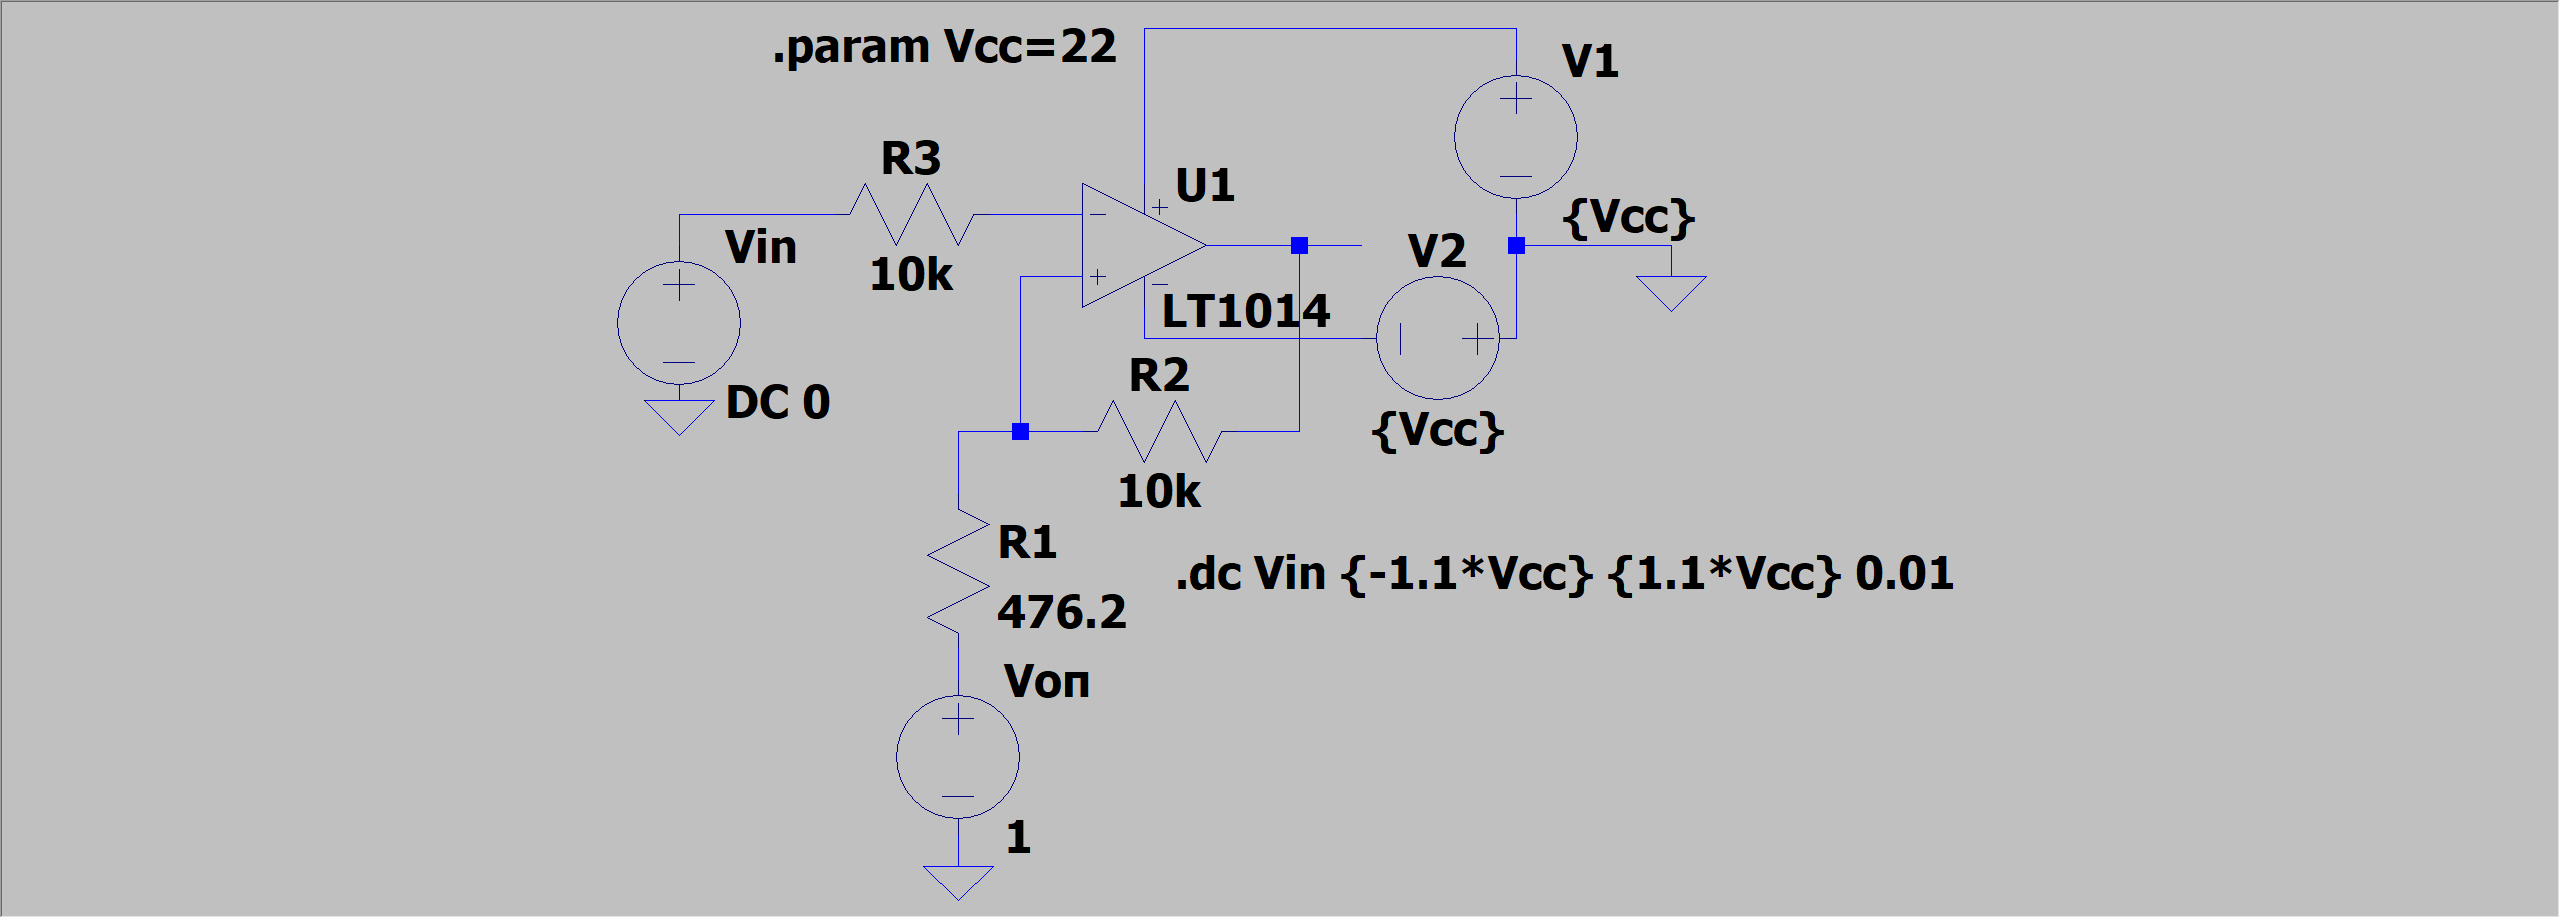
\includegraphics[scale=0.22]{scheme8.png}
        \captionsetup{skip=0pt}
        \caption{Схема двухвходового компаратора с гистерезисом на ОУ}
        \label{fig:scheme8}
    \end{figure}


    \subsection{Зависимость выходного напряжения от входного}
    Снимем зависимость $U_\text{вых}=f\left( U_\text{вх} \right)$ как в задании с ограничителем.
    Получаем
    \begin{figure}[H]
        \centering
        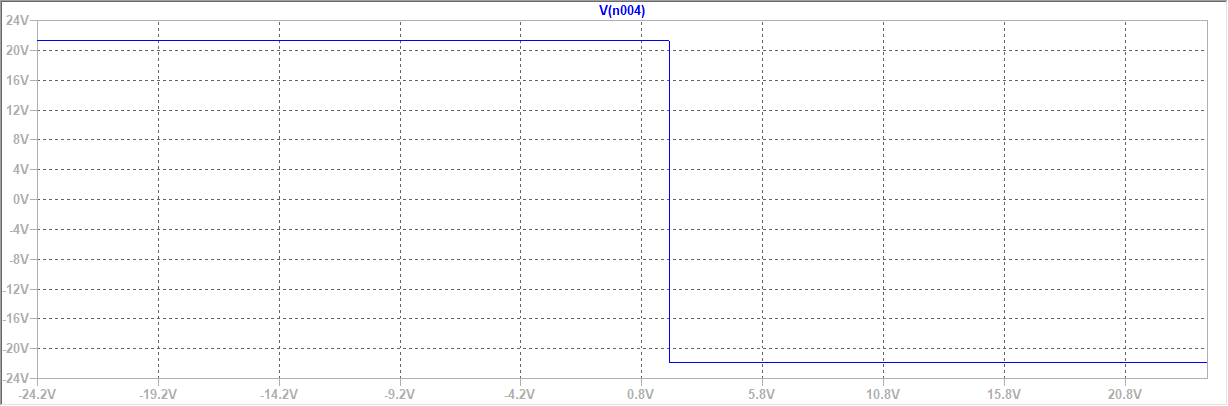
\includegraphics[scale=0.46]{6task_fuin.png}
        \captionsetup{skip=0pt}
        \caption{Выходное напряжение при $-1.1U_\text{пит}\leq U_\text{вх}\leq 1.1U_\text{пит}$ В, $U_\text{пор эксп}=1.911$ В}
        \label{fig:6task_fuin}
    \end{figure}
    \noindent Снимем зависимость $U_\text{вых}=f\left( U_\text{вх} \right)$ для гармонического
    входного воздействия амплитудой 1 В, частотой от 100 Гц до 1 кГц. Получаем (наименьший наклон
    при $f=100$ Гц -- синяя прямая, наибольший при $f=1$ кГц -- коричневая прямая)
    \begin{figure}[H]
        \centering
        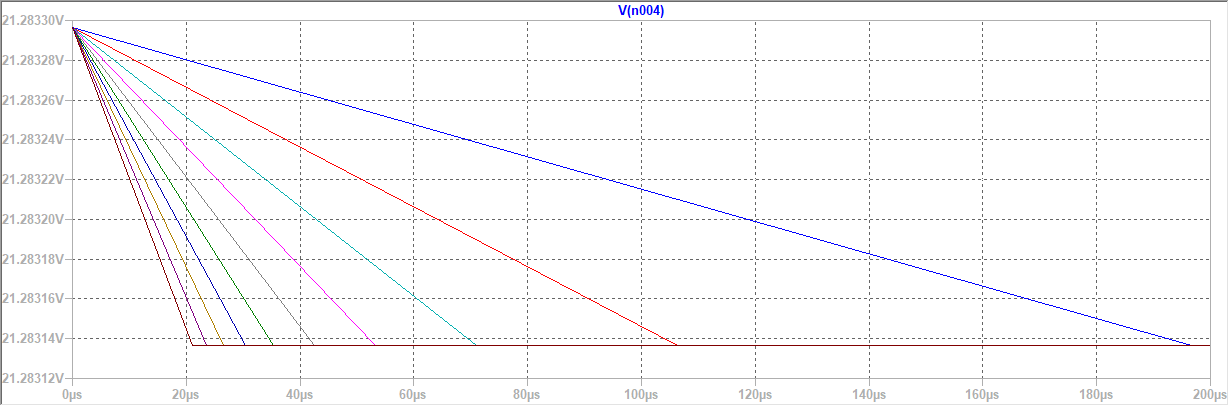
\includegraphics[scale=0.46]{6task_fuin_sine.png}
        \captionsetup{skip=0pt}
        \caption{Выходное напряжение при SINE(0 1 \{f\}), $f\in\left[ 0.1,1 \right]$ кГц, шаг $\Delta f=100$ Гц}
        \label{fig:6task_fuin_sine}
    \end{figure}
    \noindent Чем выше частота, тем больше угол наклона. Однако угол наклона имеет некоторый предел
    -- со временем он увеличивается на меньшее количество градусов.


    \subsection{Расчет параметров схемы триггера Шмитта с однополярным выходом}
    Имеем такие данные: 
    $$
    U_\text{ВТО}=5\text{ В},\ U_\text{НТО}=2\text{ В},\ U_\text{ОП}=U_\text{П}=22\text{ В},\ U_\text{нас}=U_\text{П}-1=21\text{ В},
    $$
    $$
    I_\text{дел}=1\text{ мА},\ I_\text{Н}=3\text{ мА};
    $$
    Рассчитаем $R_1,R_2,R_3,R_4,R_\text{б}$. Определим сумму $R_2+R_3$
    $$
    R_2+R_3=\dfrac{U_\text{ВТО}}{I_\text{дел}}=5\text{ кОм},
    $$
    Определим $R_1$
    $$
    R_1=\dfrac{U_\text{ОП}-U_\text{ВТО}}{I_\text{дел}}=\dfrac{22-5}{0.001}=17\text{ кОм};
    $$
    Выберем транзистор 2N2222 с $U_{\text{КЭ}_\text{нас}}=0.3$ В, $U_\text{БЭ}=0.7$ В, $h_{21_\text{min}}=50$. Определим $R_2$
    $$
    R_2=\dfrac{\left( U_\text{НТО}-U_{\text{КЭ}_\text{нас}} \right)R_1}{U_\text{ОП}-U_\text{НТО}+U_{\text{КЭ}_\text{нас}}}=\dfrac{2-0.3}{22-2+0.3}\cdot17000\approx1423.645\text{ Ом},
    $$
    Из вычисленной суммы $R_2+R_3$ выразим $R_3$
    $$
    1423.645+R_3=5000\Rightarrow R_3=3576.355\text{ Ом},
    $$
    Определим сопротивление базы транзистора
    $$
    R_\text{б}=\dfrac{U_\text{нас}-U_\text{БЭ}}{I_\text{дел}/h_{21_\text{min}}}=\dfrac{21-0.7}{0.001/50}\approx1\text{ МОм};
    $$
    Выберем стабилитрон EDZV5.1B с параметрами $U_\text{ст}=5.1$ В, $I_\text{ст}=2$ мА
    $$
    R_4=\dfrac{U_\text{нас}-U_\text{ст}}{I_\text{ст}+I_\text{Н}}=\dfrac{21-5.1}{0.002+0.003}=3180\text{ Ом}
    $$
    Таким образом, имеем
    $$
    R_1=17\text{ кОм},\ R_2\approx1.4\text{ кОм},\ R_3\approx3.6\text{ кОм},\ R_\text{б}\approx1\text{ МОм},\ R_4\approx3.2\text{ кОм};
    $$


    \subsection{Схема триггера Шмитта с однополярным выходом}
    Соберем одноименную схему согласно расчетам и варианту
    \begin{figure}[H]
        \centering
        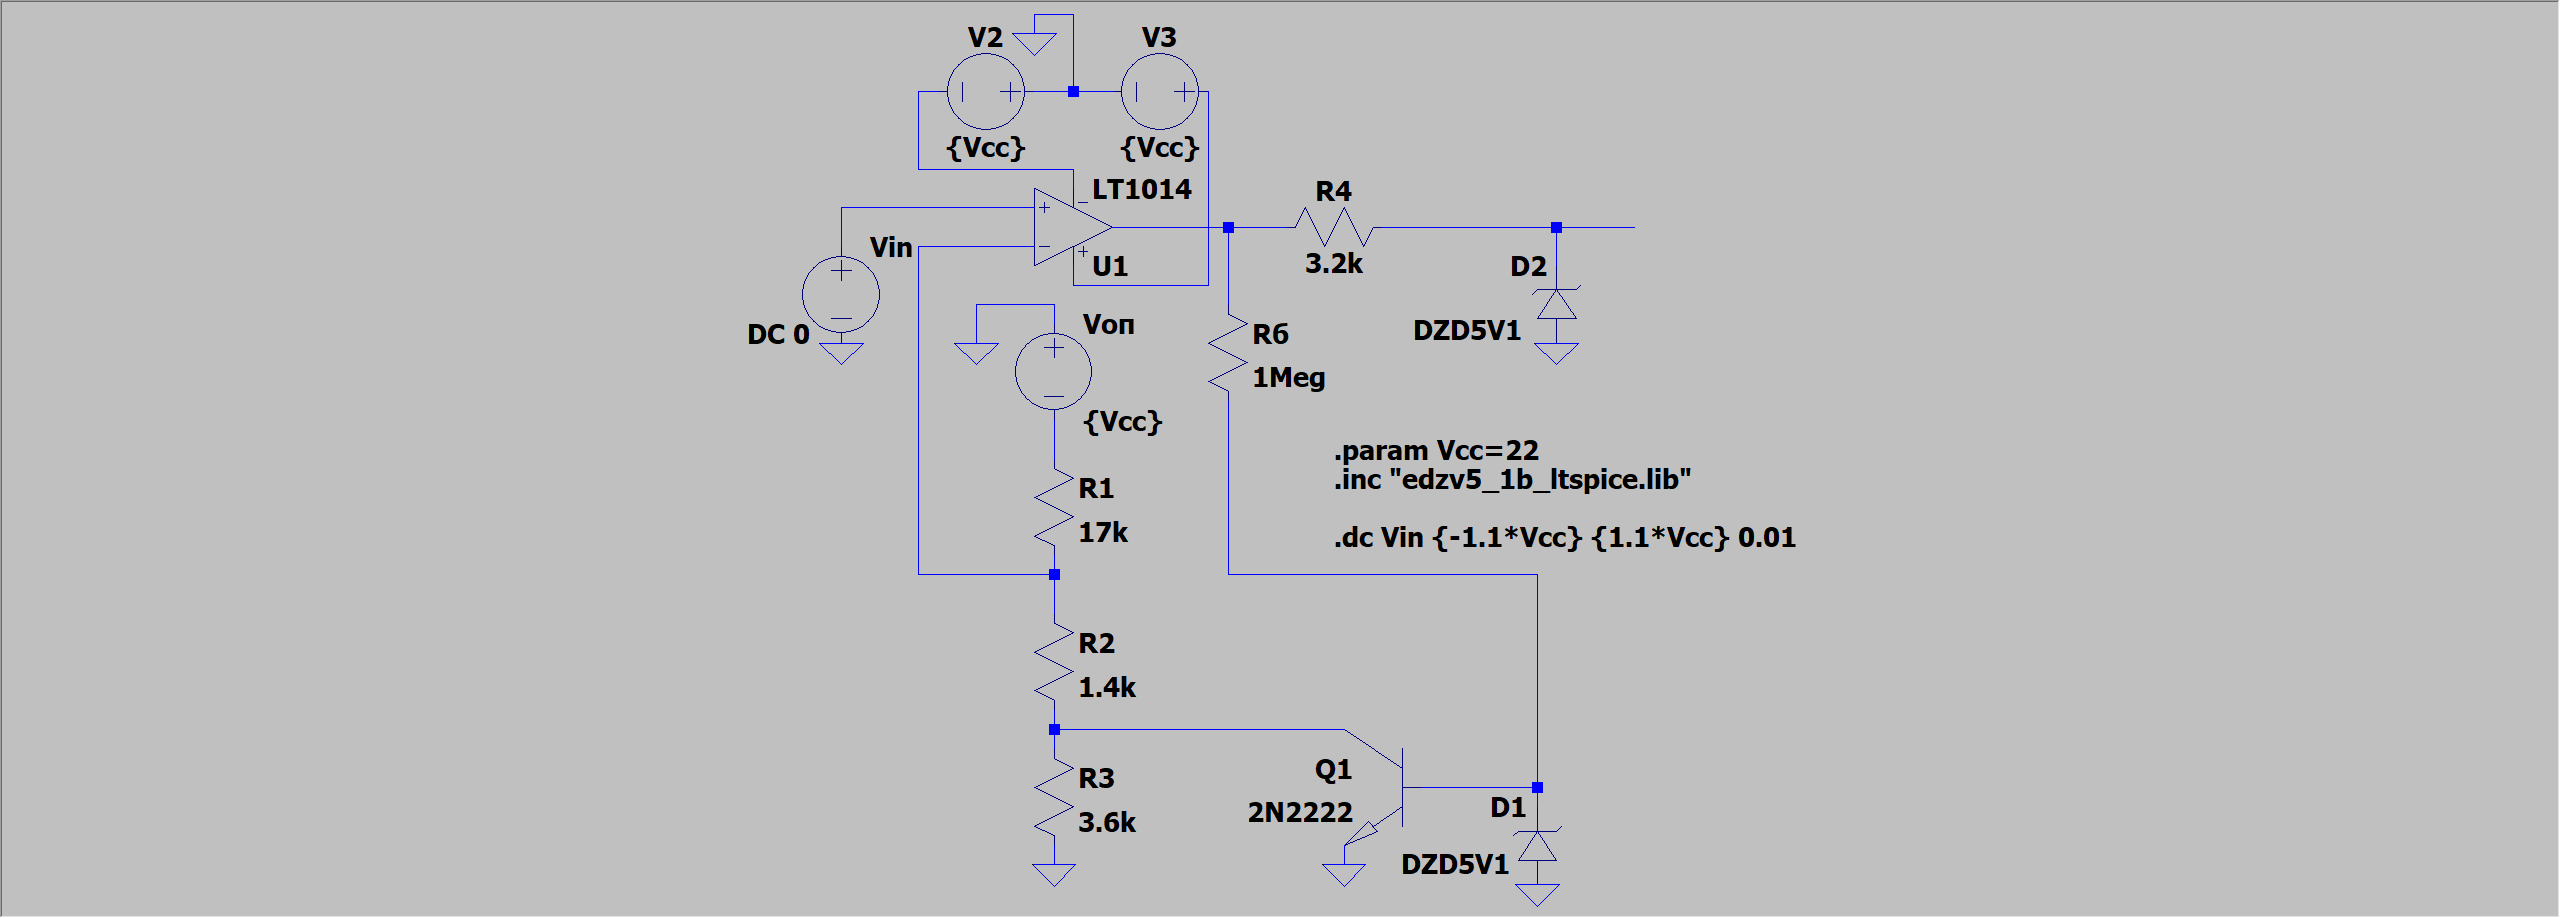
\includegraphics[scale=0.22]{scheme10.png}
        \captionsetup{skip=0pt}
        \caption{Схема триггера Шмитта с однополярным выходом}
        \label{fig:scheme10}
    \end{figure}


    \subsection{Зависимость выходного напряжения от входного}
    Снимем зависимость $U_\text{вых}=f\left( U_\text{вх} \right)$ как в задании с ограничителем.
    Получаем
    \begin{figure}[H]
        \centering
        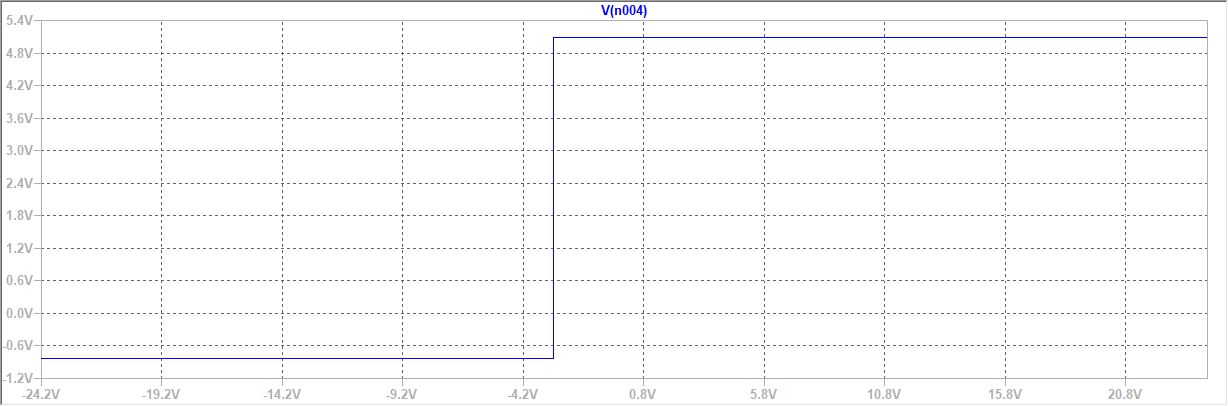
\includegraphics[scale=0.46]{7task_fuin.png}
        \captionsetup{skip=0pt}
        \caption{Выходное напряжение при $-1.1U_\text{пит}\leq U_\text{вх}\leq 1.1U_\text{пит}$ В, $U_\text{пор эксп}=-2.947$ В}
        \label{fig:7task_fuin}
    \end{figure}


    \subsection{Расчет параметров схемы компаратора с окном}
    Имеем такие данные:
    $$
    U_\text{ВТО}=7.5\text{ В},\ U_\text{НТО}=6.5\text{ В},\ U_\text{ОП}=U_\text{П}=22\text{ В},\ R_\text{Н}=2\text{ кОм},\ I_\text{дел}=5\text{ мА};
    $$
    Рассчитаем $R_1,R_2,R_3$
    $$
    R_1=\dfrac{U_\text{ОП}-U_\text{ВТО}}{I_\text{дел}}=\dfrac{22-7.5}{0.005}=2.9\text{ кОм},
    $$
    $$
    R_2=\dfrac{U_\text{ВТО}-U_\text{НТО}}{I_\text{дел}}=\dfrac{7.5-6.5}{0.005}=200\text{ Ом},
    $$
    $$
    R_3=\dfrac{U_\text{НТО}}{I_\text{дел}}=\dfrac{6.5}{0.005}=1.3\text{ кОм};
    $$


    \subsection{Схема компаратора с окном}
    Соберем одноименную схему согласно расчетам и варианту
    \begin{figure}[H]
        \centering
        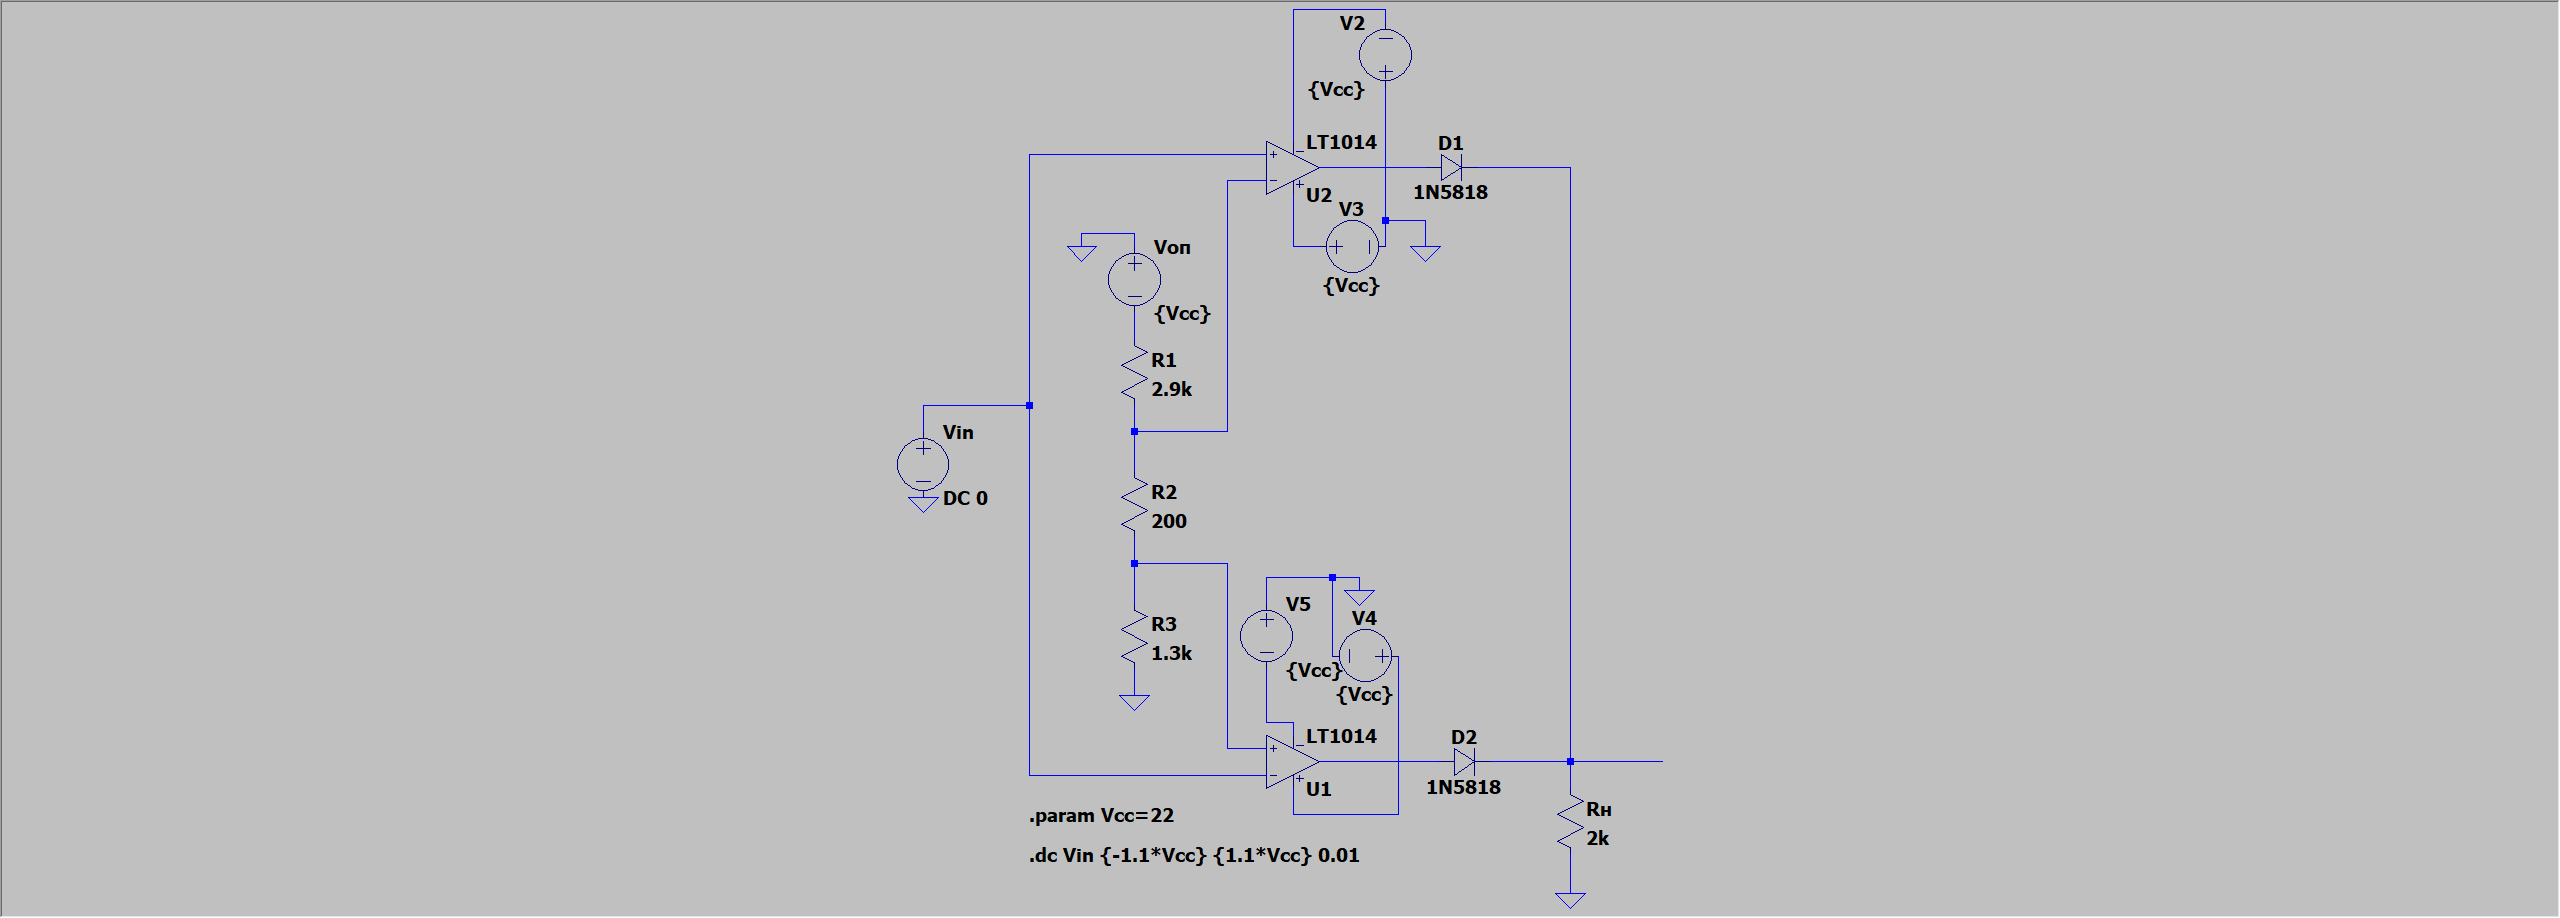
\includegraphics[scale=0.22]{scheme11.png}
        \captionsetup{skip=0pt}
        \caption{Схема компаратора с окном}
        \label{fig:scheme11}
    \end{figure}


    \subsection{Зависимость выходного напряжения от входного}
    Снимем зависимость $U_\text{вых}=f\left( U_\text{вх} \right)$ как в задании с ограничителем.
    Получаем
    \begin{figure}[H]
        \centering
        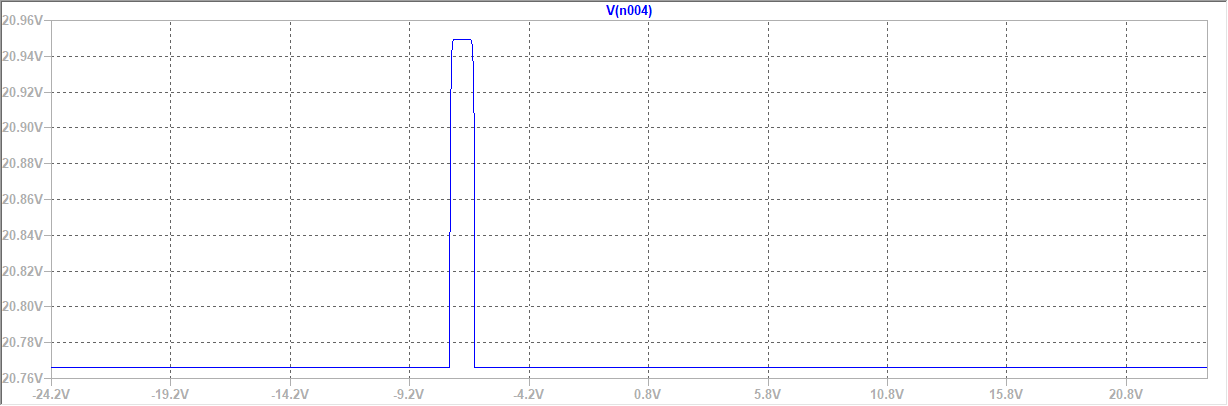
\includegraphics[scale=0.46]{8task_fuin.png}
        \captionsetup{skip=0pt}
        \caption{Выходное напряжение при $-1.1U_\text{пит}\leq U_\text{вх}\leq 1.1U_\text{пит}$ В, $U_\text{пор эксп}=\left[-7.536,-6.490\right]$ В}
        \label{fig:8task_fuin}
    \end{figure}

    
    \subsection{Вывод}
    Компараторы работает верно и подтверждают корректность расчетов и рассуждений.


    \section{Общий вывод по работе}
    В ходе лабораторной работы были рассмотрены различные схемы
    с операционными усилителями, такие как ограничитель выходного напряжения,
    нуль-компаратор, одновходовый и двухвходовый компараторы, 
    двухвходовый компаратор с гистерезисом, триггер Шмитта с однополярным выходом
    и компаратор с окном. Были промоделированы схемы, в качестве результатов
    были сняты осцилограммы выходных напряжений в зависимости от входного.
    Результаты подтвердили корректность вычислений и рассуждений.
\end{document} 